	%%%%%%%%%%%%%%%%%%%%%%%%%%%%%%%%%%%%%%%%%
%           Fichier maitre				%
%%%%%%%%%%%%%%%%%%%%%%%%%%%%%%%%%%%%%%%%%

\documentclass[a4paper, 12pt, twoside,openright]{report}

%%%%%%%%%%%%%%%%%%%%%%%%%%%%%%%%%%%%%%%%
%           Liste des packages         %
%%%%%%%%%%%%%%%%%%%%%%%%%%%%%%%%%%%%%%%%
%%%%%%%%%%%%%%%%%%%%%%%%%%%%%%%%%%%%%%%%%%%%%%%%%%%%%%%%%%%%%%%%%%%%%
\usepackage{tikz}
\usepackage{pgfplots}
%% Réglage des fontes et typo    
\usepackage[utf8]{inputenc}		% LaTeX, comprend les accents !
\usepackage[T1]{fontenc}
\usepackage{natbib}		% Doit être chargé avant babel
%\usepackage{chapterbib}
%	\renewcommand{\bibsection}{\chapter*{Références Bibliographies}}		% Met les références biblio dans un \section (au lieu de \section*)
 
\usepackage[frenchb]{babel}
\usepackage{lmodern}
\usepackage{ae,aecompl}	
\usepackage{multicol}									% Utilisation des fontes vectorielles modernes
\usepackage[upright]{fourier}
\usepackage{lipsum}
\usepackage{wrapfig}
%%%%%%%%%%%%%%%%%%%%%%%%%%%%%%%%%%%%%%%%%%%%%%%%%%%%%%%%%%%%%%%%%%%%%
% Allure générale du document
\usepackage{enumerate}
\usepackage{enumitem}
%\usepackage[section]{placeins}	% Place un FloatBarrier à chaque nouvelle section
\usepackage{epigraph}
\usepackage[font={small}]{caption}
\usepackage[francais,nohints]{minitoc}		% Mini table des matières, en français
	\setcounter{minitocdepth}{2}	% Mini-toc détaillées (sections/sous-sections)
\usepackage[notbib]{tocbibind}		% Ajoute les Tables	des Matières/Figures/Tableaux à la table des matières
%%%%%%%%%%%%%%%%%%%%%%%%%%%%%%%%%%%%%%%%%%%%%%%%%%%%%%%%%%%%%%%%%%%%%
%% Maths                         
\usepackage{amsmath}			% Permet de taper des formules mathématiques
\usepackage{amssymb}			% Permet d'utiliser des symboles mathématiques
\usepackage{mathrsfs}
\usepackage{amsfonts}			% Permet d'utiliser des polices mathématiques
\usepackage{nicefrac}			% Fractions 'inline'
\usepackage{nccmath}
%%%%%%%%%%%%%%%%%%%%%%%%%%%%%%%%%%%%%%%%%%%%%%%%%%%%%%%%%%%%%%%%%%%%%
%% Tableaux
\usepackage{multirow}
\usepackage{booktabs}
\usepackage{colortbl}
\usepackage{tabularx}
\usepackage{multirow}
\usepackage{threeparttable}
\usepackage{etoolbox}
	\appto\TPTnoteSettings{\footnotesize}
\addto\captionsfrench{\def\tablename{{\textsc{Tableau}}}}	% Renome 'table' en 'tableau'
%%%%%%%%%%%%%%%%%%%%%%%%%%%%%%%%%%%%%%%%%%%%%%%%%%%%%%%%%%%%%%%%%%%%%
%% Eléments graphiques                    
\usepackage{graphicx}			% Permet l'inclusion d'images
\usepackage{subcaption}
\usepackage{pdfpages}
\usepackage{rotating}
\usepackage{pgfplots}
	\usepgfplotslibrary{groupplots}
\usepackage{tikz}
	\usetikzlibrary{backgrounds,automata}
	\pgfplotsset{width=7cm,compat=1.3}
	\tikzset{every picture/.style={execute at begin picture={
   		\shorthandoff{:;!?};}
	}}
	\pgfplotsset{every linear axis/.append style={
		/pgf/number format/.cd,
		use comma,
		1000 sep={\,},
	}}
\usepackage{eso-pic}
\usepackage{import}
%%%%%%%%%%%%%%%%%%%%%%%%%%%%%%%%%%%%%%%%%%%%%%%%%%%%%%%%%%%%%%%%%%%%%
%% Mise en forme du texte        
\usepackage{xspace}
\usepackage[load-configurations = abbreviations]{siunitx}
	\DeclareSIUnit{\MPa}{\mega\pascal}
	\DeclareSIUnit{\micron}{\micro\meter}
	\DeclareSIUnit{\tr}{tr}
	\DeclareSIPostPower\totheM{m}
	\sisetup{
	locale = FR,
	  inter-unit-separator=$\cdot$,
	  range-phrase=~\`{a}~,     	% Utilise le tiret court pour dire "de... à"
	  range-units=single,  		% Cache l'unité sur la première borne
	  }
\usepackage[version=3]{mhchem}	% Equations chimiques
\usepackage{textcomp}
\usepackage{array}
\usepackage{hyphenat}
%%%%%%%%%%%%%%%%%%%%%%%%%%%%%%%%%%%%%%%%%%%%%%%%%%%%%%%%%%%%%%%%%%%%%
%% Navigation dans le document
\usepackage[pdftex,pdfborder={0 0 0},
			colorlinks=true,
			linkcolor=blue,
			citecolor=red,
			pagebackref=true,
			]{hyperref}	% Créera automatiquement les liens internes au PDF
					% Doit être chargé en dernier (Sauf exceptions ci-dessous)
%%%%%%%%%%%%%%%%%%%%%%%%%%%%%%%%%%%%%%%%%%%%%%%%%%%%%%%%%%%%%%%%%%%%%
%% Packages qui doivent être chargés APRES hyperref	             
\usepackage[top=2.5cm, bottom=2cm, left=3cm, right=2.5cm,
			headheight=15pt]{geometry}
\usepackage{fancyhdr}
\addtolength{\headheight}{2.5pt}
\fancyhf{}
%\fancyhead[LE,RO]{\nouppercase{\thepage}}
%\fancyhead[L]{\nouppercase{\leftmark}}
\renewcommand{\headrulewidth}{2pt}
\renewcommand{\footrulewidth}{1pt}
\pagestyle{fancy}
\lhead{\nouppercase{\leftmark}}
\rfoot{page \centering \thepage}
\pagestyle{fancy}
\usepackage{tcolorbox}
\usepackage[acronym,xindy,toc,numberedsection,ucmark]{glossaries}
	\newglossary[nlg]{notation}{not}{ntn}{Notation} % Création d'un type de glossaire 'notation'
	\makeglossaries
	\loadglsentries{Glossaire}			% Utilisation d'un fichier externe pour la définition des entrées 
\usepackage{float}% http://ctan.org/pkg/float
\usepackage[linesnumbered,ruled,vlined]{algorithm2e}
\usepackage{algpseudocode}

\usepackage{etex}   

\pgfplotsset{every axis/.append style={
		axis x line=middle,    % put the x axis in the middle
		axis y line=middle,    % put the y axis in the middle
		axis line style={<->}, % arrows on the axis
		xlabel={$x$},          % default put x on x-axis
		ylabel={$y$},          % default put y on y-axis
	},
	cmhplot/.style={color=blue,mark=none,line width=1pt,<->},
	soldot/.style={color=red,only marks,mark=*},
	holdot/.style={color=green,fill=white,only marks,mark=*},
}

\tikzset{>=stealth}


		% Liste des packages et de leurs options
%%%%%%%%%%%%%%%%%%%%%%%%%%%%%%%%%%%%%%%%
%           Commandes perso            %
%%%%%%%%%%%%%%%%%%%%%%%%%%%%%%%%%%%%%%%%

\newcommand{\alp}{\texorpdfstring{\ensuremath{\upalpha}\xspace}{alpha }}
\newcommand{\bet}{\texorpdfstring{\ensuremath{\upbeta}\xspace}{b\'{e}ta }}
\newcommand{\alpbet}{\texorpdfstring{\ensuremath{\upalpha-\upbeta}\xspace}{alpha-b\'{e}ta}}
\newcommand{\alpt}{\ensuremath{\alpha_2}\xspace}
\newcommand{\strt}{\gls{strt}\xspace}


% Tenseur des déformation cylindrique
\newcommand{\epsrr}{\ensuremath{\varepsilon_{rr}}\xspace}
\newcommand{\epstt}{\ensuremath{\varepsilon_{\theta\theta}}\xspace}
\newcommand{\epszz}{\ensuremath{\varepsilon_{zz}}\xspace}
\newcommand{\epsrt}{\ensuremath{\varepsilon_{r\theta}}\xspace}
\newcommand{\epstz}{\ensuremath{\varepsilon_{\theta z}}\xspace}
\newcommand{\epszr}{\ensuremath{\varepsilon_{zr}}\xspace}

\newcommand{\matlab}{\textsc{Matlab}\texttrademark\xspace}



%% Figures centrées, et en position 'here, top, bottom or page'
\newenvironment{figureth}{%
		\begin{figure}[htbp]
			\centering
	}{
		\end{figure}
		}

		
%% Tableaux centrés, et en position 'here, top, bottom or page'
\newenvironment{tableth}{%
		\begin{table}[h]
			\centering
			%\rowcolors{1}{coleurtableau}{coleurtableau}
	}{
		\end{table}
		}


%% Sous-figures centrées, en position 'top'		
\newenvironment{subfigureth}[1]{%
	\begin{subfigure}[t]{#1}
	\centering
}{
	\end{subfigure}
}

\newcommand{\citationChap}[2]{%
	\epigraph{\og \textit{#1} \fg{}}{#2}
}

%% On commence par une page impaire quand on change le style de numérotation de pages 
\let\oldpagenumbering\pagenumbering
\renewcommand{\pagenumbering}[1]{%
	\cleardoublepage
	\oldpagenumbering{#1}
}

\newcommand{\mcd}{model checking distribué}
\newcommand{\mc}{model checking}
\newcommand{\border}{\emph{Border}}
\newcommand{\ssti}{Search\_ States\_ To\_ Impor}
\newcommand{\notifier}{\emph{Notifier}}
\newcommand{\bn}{\emph{\border{} et \notifier{}}}

\newcommand{\ei}{Etat Interne}
\newcommand{\CDS}{CDS}
\newcommand{\CDSDef}{Comportemental Distribution States}
\newcommand{\ee}{Etat Externe}
\newcommand{\deplacer}{déplacer}
\newcommand{\dupliquer}{dupliquer}
\newcommand{\parametreone}{\alpha}
\newcommand{\parametretwo}{\beta}
\newcommand{\parametretree}{\gamma}
\newcommand{\parametrefive}{\delta}
\newcommand{\parametrefour}{\gamma m}
\newcommand{\ministere}{R\'{e}publique  Alg\'{e}rienne D\'{e}mocratique et Populaire Minist\'{e}re de  l'enseignement Sup\'{e}rieur et de la Recherche Scientifique Faculté des Nouvelles Technologies de l'Information et la Communication Département d’Informatique Fondamentale et ses Applications}
\newcommand{\sneuf}{\og S9 \fg{}}
\newcommand{\s}[1]{\og #1 \fg{}}
\newcommand{\mone}{\og machine 1 \fg{}}
\newcommand{\mi}{\og machine i \fg{}}
\newcommand{\mj}{\og machine j \fg{}}
\newcommand{\mtwo}{\og machine 2 \fg{}}
\newcommand{\mtree}{\og machine 3 \fg{}}
\newcommand{\curenti}{curent_{iteration}}
\usepackage{amsmath,amsthm}
\usepackage{thmtools}
\theoremstyle{remark}
\newtheorem{Exemple}{Exemple}[section]
\newtheorem{theorem}{Theorem}
\theoremstyle{definition}
\newtheorem{definition}[theorem]{Définition}
\newtheorem{etape}[theorem]{Étape}

\newcommand{\mysection}[2][]
   {\section[#1]
     {\centering #2}
       \setcounter{figure}{0}
       \renewcommand{\thefigure}{\thesection.\arabic{figure}} %Arabic figures
       \renewcommand{\thesection}{\Roman{section}}               %Roman numeral title
}
\newcommand{\mysectionNoNumerotation}[2][]
   {\section[#1]
     {#2}
       \renewcommand{\thesection}{{section}}               %Roman numeral title
}
\setcounter{secnumdepth}{3} 
%Subsections do not get centered
\allowdisplaybreaks
\newcommand{\mysubsection}[2][]
{\renewcommand*{\thesubsubsection}{\alph{subsubsection}}
\subsubsection[#1]{#2} 
}
\newcommand{\sectionbreak}{\clearpage}
\algnewcommand\algorithmicforeach{\textbf{for each}}
\algdef{S}[FOR]{ForEach}[1]{\algorithmicforeach\ #1\ \algorithmicdo}

\SetNlSty{}{}{}
\let\oldnl\nl% Store \nl in \oldnl
\newcommand\nonl{%
  \renewcommand{\nl}{\let\nl\oldnl}}% Remove line number for one line


\usepackage{float}

\floatstyle{ruled}
\newfloat{function}{thp}{lop}
\floatname{function}{Function}
\newfloat{procedure}{thp}{lop}
\floatname{procedure}{Procedure}

\newcommand{\frenchAbstract}[1]{\gdef\@frenchAbstract{#1}} 
\newcommand{\frenchAbstractKeywords}[1]{\gdef\@frenchAbstractKeywords{#1}} 

\newcommand{\englishAbstract}[1]{\gdef\@englishAbstract{#1}} 

\newcommand{\englishAbstractKeywords}[1]{\gdef\@englishAbstractKeywords{#1}} 


 %================= configuring minitoc ==================%

%% disabling chapter numbers
\newcommand{\filterminitoc}[1]{#1}
\renewcommand{\thesection}{\csname filterminitoc \endcsname{\arabic{chapter}.}\arabic{section}}
\newcommand{\minitocsection}{\begingroup\renewcommand{\filterminitoc}[1]{}\minitoc\endgroup}
%=============== Customizing Chapters Names ===============%
%@author: Stoufa
%Package pstcol Warning:
%************************************
%(pstcol) The package `pstcol' is obsolet!
%(pstcol) You should use `pstricks' directly:
%(pstcol) \usepackage{pstricks}
%(pstcol) ************************************
%\usepackage{pstcol}
\usepackage{pstricks}
\makeatletter
\def\thickhrulefill{\leavevmode \leaders \hrule height 1.2ex \hfill \kern \z@}

\def\@makechapterhead#1{
	\vspace*{30\p@}%
	{\parindent \z@ \centering \reset@font
		\thickhrulefill\quad 
		\scshape\bfseries\textit{\@chapapp{}  \thechapter}  
		\quad \thickhrulefill
		\par\nobreak
		\vspace*{10\p@}%
		\interlinepenalty\@M
		\hrule
		\vspace*{10\p@}%
		\Huge \bfseries #1 \par\nobreak
		\par
		\vspace*{10\p@}%
		\hrule
		\vskip 50\p@
	}
	\minitocsection
	\thispagestyle{empty}%
	\newpage
}
\def\@makeschapterhead#1{\hbox{%
		\huge\hbox{\textbf{#1}}%
	}\par\vskip 1cm}	% Commandes et environnements perso

%%%%%%%%%%%%%%%%%%%%%%%%%%%%%%%%%%%%%%%%%%
%           Page de Garde		         %
%%%%%%%%%%%%%%%%%%%%%%%%%%%%%%%%%%%%%%%%%%

\makeatletter
 
\def\@specialite{Spécialité}
\newcommand{\specialite}[1]{
  \def\@specialite{#1}
}

\def\@directeur{directeur}
\newcommand{\directeur}[1]{
  \def\@directeur{#1}
}

\def\@encadrant{encadrant}
\newcommand{\encadrant}[1]{
  \def\@encadrant{#1}
}
\def\@jurya{}{}{}
\newcommand{\jurya}[3]{
  \def\@jurya{#1,	& #2	& #3\\}
}
\def\@juryb{}{}{}
\newcommand{\juryb}[3]{
  \def\@juryb{#1,	& #2	& #3\\}
}
\def\@juryc{}{}{}
\newcommand{\juryc}[3]{
  \def\@juryc{#1,	& #2	& #3\\}
}
\def\@juryd{}{}{}
\newcommand{\juryd}[3]{
  \def\@juryd{#1,	& #2	& #3\\}
}
\def\@jurye{}{}{}
\newcommand{\jurye}[3]{
  \def\@jurye{#1,	& #2	& #3\\}
}
\def\@juryf{}{}{}
\newcommand{\juryf}[3]{
  \def\@juryf{#1,	& #2	& #3\\}
}
\def\@juryg{}{}{}
\newcommand{\juryg}[3]{
  \def\@juryg{#1,	& #2	& #3\\}
}
\def\@juryh{}{}{}
\newcommand{\juryh}[3]{
  \def\@juryh{#1,	& #2	& #3\\}
}
\def\@juryi{}{}{}
\newcommand{\juryi}[3]{
  \def\@juryi{#1,	& #2	& #3\\}
}
\makeatother 
\newcommand\EtiquetteThese{%
	\put(-10,10){%
		\parbox[t][\paperheight]{\paperwidth}{%
			\hfill
			\colorbox{black}{		
				\begin{minipage}[b]{3em}
					\centering\Huge\textcolor{white}{M\\A\\S\\T\\E\\R\\}
					\vspace{0.3cm}
				\end{minipage}
			}
		}
	}
}

\makeatletter
\newcommand{\pagedegarde}{
\newgeometry{top=2.5cm, bottom=2cm, left=2cm, right=1cm}
 
\AddToShipoutPicture*{\EtiquetteThese}
  \begin{titlepage}
	\centering	

 \begin{tableth}
	\centering
	\begin{tabular}{*{3}{c}}
		\begin{minipage}{0.2\textwidth}
				
\includegraphics[width=0.7\linewidth]{img/uc2.png}
			\end{minipage}
			&	\begin{minipage}{0.5\textwidth}
				\begin{center}
					\vspace{0.5cm}
						  \ministere{}
				\end{center}				
			\end{minipage}	&
			\begin{minipage}{0.2\textwidth}
				
\includegraphics[width=0.7\linewidth]{img/uc2.png}
			\end{minipage}\\

	\end{tabular}	
\end{tableth}

    \vspace{1cm}
    	\begin{minipage}{1\textwidth}\raggedright
			 {\Large Ann\'{e}e  : }\\
			 {\Large \No d'ordre    : }\\
			 {\Large Série : }\\
		\end{minipage}	
 
    \vspace{0.5cm}
      
    	{\Large{\textbf{M\'EMOIRE}}}\\
    	\vspace{0.5cm}
    	\textit{pour obtenir le diplôme}\\
    	\vspace{0.5cm}
    	{\Large{\textbf{MASTER en Informatique}}}\\
    	\vspace{0.5cm}
    	 {\textbf{Option :} Réseaux et Systèmes Distribués}\\
    \vspace{0.5cm}
    \begin{tcolorbox}[colback=white,boxrule=0pt,toprule=3pt,bottomrule=3pt,arc=0pt,top=0mm,right=0mm,left=0mm,bottom=0mm,boxsep=0.5mm]{
    		\begin{tcolorbox}[colback=white, boxrule=0pt,toprule=1pt,bottomrule=1pt,arc=0pt,enlarge bottom by=-0.9mm, auto outer arc]
    			\centering
    			{\huge\textbf{\@title}}
    		\end{tcolorbox}
    	}
    \end{tcolorbox}
    \vspace{0.5cm}
    	\textit{ Présenté et soutenu publiquement par}\\
    \vspace{0.5cm}
    	{\Large {\bfseries \@author}} \\
    \vspace{0.5cm}
    	le \@date \\   
    
    \vspace{1cm}
	\begin{tabular}{>{\bfseries}llr}
		\large Jury\\
		%Directeur de mémoire : {\bfseries \@directeur}\\
		%Co-encadrant de mémoire : {\bfseries \@encadrant}\\
		\@jurya
		\@juryb
		\@juryc
		\@juryd
	\end{tabular}
	\vfill 
  \end{titlepage}
\nopagebreak
\restoregeometry  
\nopagebreak  
}
\makeatother
\nopagebreak
 
%%%%%%%%%%%%%%%%%%%%%%%%%%%%%%%%%%%%%%%%%%%%%%%%%%%%%%%%%%%%%%%%%
%%   			Liste des fichiers à compiler					%
 %%%%%%%%%%%%%%%%%%%%%%%%%%%%%%%%%%%%%%%%%%%%%%%%%%%%%%%%%%%%%%%%%
%	\includeonly{Chapitre1,Chapitre2,Annexes}

% Infos de la page de garde
\author{Karimou Seyni Ibrahim}
\title{Distribution des Espace Etats}
\specialite{Réseaux et Système Distribué}
\directeur{...}
\encadrant{...}
\date{\today}
\jurya{...}
\juryb{...}

% Méta-données du PDF
\hypersetup{
    pdfauthor={\@author},
    pdfsubject={Manuscrit de Master},
    pdftitle={\@title},
    pdfkeywords={space d'états, distribution, modèle checker}
}

\begin{document}
	\let\cleardoublepage\clearpage
% Préambule	
	\pagedegarde	
	\pagenumbering{roman}
	% Table des matières
		\setcounter{tocdepth}{1}	% Pas besoin de trop détailler le sommaire ici (chapitres/sections)
		\dominitoc						% Génération des mini-toc	\pagenumbering{arabic}
		\tableofcontents
	% Liste des figures
		\renewcommand*\listfigurename{Liste des figures}
		\listoffigures
	% Liste des tableaux
	\listoftables

%%%%%%%%%%%%%%%%%%%%%%%%%%%%%%%%%%%%%		
%        Contenu du document        %
%%%%%%%%%%%%%%%%%%%%%%%%%%%%%%%%%%%%%
 
	\setcounter{mtc}{3}	% "Corrige" les minitocs décallés à cause des chapter* (ex : table des matières)
	\pagenumbering{gobble}
\chapter*{}
\vspace{4mm}

\begin{flushright}
	\large
	\textbf{
		A ma mère \\
		A mon père \\
		A toute ma famille\\ A mes ami(e)s
	} 
\end{flushright}

\vspace{8mm}
\chapter*{Remerciements}
Je tiens tout d’abord à remercier Allah, le Clément, le miséricordieux qui nous a permis de mener à bien ce modeste travail.
\\\\
En premier lieu, je tiens à exprimer ma sincère gratitude à mon encadreur\\ \textbf{\saidouni{}}, pour son intégrité, sa disponibilité, sa générosité de partager ses connaissances. Je voudrais lui témoigner ici toute ma gratitude pour m'avoir guidé durant ces périodes et laisse entrevoir ce que le mot recherche veut dire.
\\\\
Je remercie chaleureusement \textbf{\bouneb{}} pour avoir accepté d'être mon co-encadreur, pour son soutien, ses nombreux conseils et l'intérêt qu'il a porté à mon travail.
\\\\
Je souhaite exprimer toutes ma reconnaissance à mes parents qui m'ont soutenu tout au long de ces années et m'ont toujours encouragé de faire ce que je souhaitais et de donner le meilleur de moi-même. 
\\\\
Mes plus vifs remerciements s’adressent à tous les corps enseignants pour leur patience, leur dévouement pour nous avoir apporté le bagage nécessaire.
\\\\
Je voudrais aussi exprimer mon amitié aux personnes avec qui j'ai eu le plaisir de partager ses années d'études et surtout ceux du premier et du second cycle.

	
	\pagenumbering{gobble}
\chapter*{}
\begin{changemargin}{3mm}{0cm}
    \begin{minipage}[c]{0.96\columnwidth}        

        \selectlanguage{french}
        
        {\LARGE\textbf{Résumé}}
        \vskip1mm
            \begingroup
                La vérification formelle constitue une étape indispensable pour garantir le bon fonctionnement des systèmes complexes et critiques. Le model checking est une technique efficace pour vérifier des propriétés sur des systèmes décrit avec un modèle formel. Ce pendant, cette méthode de vérification souffre d'un problème majeur engendré par l'explosion combinatoire de l'espace d'états à explorer  dans un temps raisonnable.
                \\\\
                Pour merdier a ce problème, la distribution de l'espace d'états est la solution la plus rependus  en vue de tirer profit de la quantité de mémoire et de la puissance de calcul disponibles sur chaque machine. Par contre aboutir à une meilleur distribution pour accélérer la vérification s'avère être difficile a réalisé.\\
                
                Notre travail réside dans la distribution de l'espace d'états, pour établir un compromis entre l’équilibrage de charge des différentes machines et la minimisation du taux de communications. Pour cela, nous proposons une nouvelle approche de distribution en avale de l'espace d'états basée la théorie de jeux et l'analyse des états. L’approche proposée vise à analyser l'espace d’états tout en extrayant les informations pertinentes sur les états. Ensuite, redistribuer les états suite à leurs pertinences soit migrés définitivement soit dupliqués sur d’autres machines, afin de minimiser le nombre de communications entre les machines. Cela est fait grâce à une stratégie comportementale de la théorie de jeux au quelle les machines cherchent à optimiser leur taux de communications tout en maintenant l'équilibrage de charge entre les machines à l’aide de seuils prédéfinis pour chaque machine. Ceci permet à une application d'optimiser ses comportements en cumulant ses expériences d’exécutions, ainsi grâce à l'utilisation des bases de données orientés graphes, les prochaines exécutions de l’application seront fait à partir des améliorations gagnées précédemment.
            \endgroup
        \vskip1mm
        {\textbf{Mots clés : }
            \begingroup
                Réseau de Petri, Calcul parallèle, Structure de Kripke Distribué, Model checking distribué, Distribution des espaces d'états, 
                Génération de l’espace d’états, Méthodes d’optimisation, Théorie de jeux.
            \endgroup
        }
    \end{minipage}    
\end{changemargin}
\break
        
\pagenumbering{gobble}
\chapter*{}
\begin{changemargin}{3mm}{0cm}
	\begin{minipage}[c]{0.96\columnwidth} 
		\selectlanguage{english}
		{\LARGE\textbf{Abstract}}
		\vskip1mm
		\begingroup
		Formal verification is an essential step for ensuring the proper functioning of complex and critical systems. Model checking is an effective technique for checking properties on systems described with a formal model. However, this verification method suffers from a major problem caused by the combinatorial explosion of the state space to be explored in a reasonable time.
		\\
		
		To solve this problem, the states space distribution is the most common solution to take advantage of the amount of memory and computing power available on each machine. On the other hand, it is difficult to obtain a better distribution to accelerate the calculation of the verification.
		\\\\
		Our work lies in the distribution of states space, to establish a compromise between the load balancing of the different machines and the minimization of the communication rate. For this, we propose a new distribution approach in downstream of the states space based game theory and state analysis. The proposed approach aims to analyze the states space while extracting relevant state information. Then, redistribute the states following their relevance either migrated permanently or duplicated on other machines, in order to minimize the number of communications between the machines. This is done through a behavioral strategy of game theory in which machines seek to optimize their communications rate while maintaining load balancing between machines using predefined thresholds for each machine. This allows an application to optimize its behavior by combining its execution experiences, and thanks to the use of graph-oriented databases, the next executions of the application will be made from the improvements previously gained.		
		\endgroup
		\vskip1mm
		{\textbf{Keywords : }
			\begingroup			
			Petri Net, Parallel Computing, Distributed Kripke Structure, Distributed Model Checking, State Space Distribution,	State Space Generation, Optimization Methods, Game Theory.
			\endgroup
		}
    \end{minipage}    
\end{changemargin}	
	\pagenumbering{arabic}
	%%%%%%%%%%%%%%%%%%%%%%%%%%%%%%%%%%%%%%%%%%%%%%%%%%%%%%%%%%%%%%%%%%%%%%%%%%%%%%%%%%%%%%%%%%%%%
%%									Chapitre Introduction
%%%%%%%%%%%%%%%%%%%%%%%%%%%%%%%%%%%%%%%%%%%%%%%%%%%%%%%%%%%%%%%%%%%%%%%%%%%%%%%%%%%%%%%%%%%%%
\chapter{Introduction Générale}
\section{Introduction}
Depuis la découverte de l’informatique, de nombreuses activités de la vie courante ont été simplifiés. Aujourd’hui, on se sert de l’informatique pour traiter des informations en utilisant des logiciels et des réseaux informatiques. Et pour ce faire, ce système est devenu maniable presque dans tout le domaine de la vie courante (L'alimentation, L'eau, L’entretien de la maison, La construction, Le bénévolat, Le jardinage, Les achats, Les loisirs, avionique, ferroviaire, nucléaire, médicale, etc.).

Les systèmes(avionique, ferroviaire, nucléaire, médicale, etc.) sont caractérisés par leurs aspects critiques, complexes et réactifs, et opèrent comme des programmes très concurrents avec des milliers d’entités s’exécutant en parallèle et communiquant sous différentes conditions environnementales. L’analyse de ces systèmes est particulièrement difficile, car un mauvais fonctionnement du système aurait un impact important sur la sécurité ou la vie des personnes, des entreprises ou des biens. En fait, plusieurs catastrophiques sont dues à des erreurs de spécification, a titre d'exemple, l'échec du vol inaugural de la fusée Ariane 5 en 1996 a pour origine  plusieurs erreurs de spécification du logiciel de commande, et notamment de son système de tolérance aux faute \cite{arian5}, en 2002, autre exemple dramatique, celui d’un missile anti-missile Patriot déployé en Arabie Saoudite, que le système de surveillance a refusé de lancer sur un missile ennemi \cite{patriot}, le bug de l'an 2000 est un exemple, causé par une erreur de vérification sur les dates \cite{bug2000}.

Les méthodes formelles permettent de parvenir à une preuve, au sens mathématique, le bon fonctionnement du système. Ils
se basent sur la description du système avec un langage formel (i.e. non ambigu) muni d’une sémantique précise, une fois le système décrit, ces méthodes peuvent prouver la correction du modèle en assurant que le comportement du système développé satisfait tous les besoins désirés et les propriétés spécifiées. Cette vérification peut prendre plusieurs formes, dont l’approche basée sur la preuve de théorèmes permet de vérifier de manière paramétrique un système qui est décrit sous la forme d’axiomes \cite{Rushby2001}, et l’approche basée sur le model checking, il permet de confronter un système (sa description opérationnelle) à ses spécifications (les propriétés que l’on attend de lui), de détecter automatiquement des erreurs dans le processus de conception \cite{Clark1999}.

Les techniques des méthodes formelles sont automatisable dès lors que l’on possède un modèle formel et des propriétés à vérifier. La puissance de cette méthode réside dans la précision de la réponse obtenue (la propriété est vérifiée ou non),  aussi elle fournit un contre-exemple en cas d’erreur dans le modèle (le système ne vérifie pas la propriété spécifiée) permettant ainsi de corriger le problème.

\section{Problématique}
Du fait de la taille de l'espace d'états de certains systèmes spécifier, il est en général impossible de les explorer dans un temps raisonnable ou il se heurte au problème de l'explosion combinatoire du nombre d'états à explorer. Ce problème est retardé par la distribution de l'espace d'états sur un réseau de machines connectées afin de tirer profit de la quantité de mémoire et de la puissance de calcul disponibles.

Dans l’implémentation distribuée, le model checking souffre un problème majeur engendré par la distribution de l'espace d'états du systèmes spécifier car il est impossible de connaître à l’avance le temps de calcul que prendra l’exploration de l'espace d'états. L'espace d'états est distribué de sorte que des machines pourraient avoir des états trop faciles à calculer. Il est donc difficile de s’assurer que toutes les machines sont utilisées au maximum de
leur capacité et donc on ne peut pas arriver à une accélération linéaire.

Notre objectif dans la génération distribuée est d’établir un compromis entre l’équilibrage de la charge entre les différentes machines et la minimisation des coûts de communication. Cependant, l’expérience pratique a montré qu’aucun de ces deux objectifs pris séparément ne peut suffire pour avoir une bonne distribution de l’espace des états.

\section{Contributions}

Dans l’implémentation distribuée, les solutions proposées dans la littérature travaillent en amont c-à-d avant
ou au moment de la génération de l’espace d’états en utilisant des fonctions de partitions. La philosophie de ces méthodes visent à aboutir à la meilleure distribution sans savoir au préalable les applications qui vont exploiter le graphe distribué par la suite. Cependant ces applications sont de nature différentes, et peuvent dans le cas échéant être inconnues. Suite à cela, nous proposons une nouvelle approche de distribution en avale de l'espace d'états basée sur le comportement des applications. L’approche proposée vise à analyser le comportement d’un système donné en générant son espace d’état et en extrayant les informations pertinentes sur les états et leurs connexions (transitions internes et externes). Ensuite, redistribuer l’espace d’états selon certaines heuristiques afin d’optimiser les performances du système. Cela est fait en définissant une bonne localité pour l'état comme celle qui optimise à la
fois l’équilibre de charge et la quantité de communication entre les machines. L’intuition derrière cette approche permet à une application d'optimiser ses comportements en cumulant ses expériences d’exécution, ainsi grâce à l'utilisation des base de donnée orienté graphe, les prochaines exécutions future de l’application seront fait à partir des améliorations gagnés précédemment.

\section{Plan du document}
Conformément à ce qui vient d’être exposé dans notre travail de recherche, il se décompose en deux parties :

\paragraph{La première partie} est consacrée à la présentation du domaine de notre étude et les
principaux concepts utilisés dans ce travail. Elle contient deux chapitres.
\begin{description}
	\item[Le premier chapitre] aborde quelques notions de base sur l’optimisation combinatoire ainsi que de la théorie de graphes. Introduit les notion de distribution de l'espace d'états et pressente les implémentations distribuées du model checking proposées dans la littérature.
	\item [Le deuxième chapitre ] est consacré à la présentation du contexte général de notre travail, introduit les réseaux de Petri ainsi que les systèmes de transitions étiquetées et les structures de Kripke, ensuite met l’accent sur	la technique de model checking en pressentant les concepts de la logique temporaire arborescente. Par la suite, le model cheching distribué est présenté.
\end{description}

\paragraph{La seconde partie} est dédiée aux contributions de notre étude, Elle contient uns chapitre.
 Nous présentons notre approche l’algorithme de génération parallèle d'une structure de Kripke distribué à partir d'un réseau de Petri. Ensuite, nous décrivons notre approche de distribution en avale de l'espace d'états par le comportement des applications. Nous finirons avec la présentation d'un système de stockage dédiée aux espace d'états et l’implémentation de cette approche ainsi que l’interprétation des résultats obtenus.
 \\\\
 
 
Enfin, la conclusion générale qui englobe l’aboutissement des résultats obtenus  ainsi que les perspectives à développer dans l’avenir.  


	\clearpage
 	\part{Contexte de travail}
	\clearpage
	\nopagebreak
		%%%%%%%%%%%%%%%%%%%%%%%%%%%%%%%%%%%%%%%%%%%%%%%%%%%%%%%%%%%%%%%%%%%%%%%%%%%%%%%%%%%%%%%%%%%%%
%%									Chapitre Approche de partitionnement et de distribution des graphes
%%%%%%%%%%%%%%%%%%%%%%%%%%%%%%%%%%%%%%%%%%%%%%%%%%%%%%%%%%%%%%%%%%%%%%%%%%%%%%%%%%%%%%%%%%%%%
\chapter{Approche de partitionnement et de distribution des graphes}
	\citationChap{
	...
	}{...}
	\minitoc
	\newpage

%%%%%%%%%%%%%%%%%%%%%%%%%%%%%%%%%%%%%%%%%%%%%%%%%%%%%%%%%%%%%%%%%%%%%%%%%%%%%%%%%%%%%%%%%%%%%
\section{Introduction} 
Depuis le problème des ponts de Königsberg \citep{EULER1736}, la théorie des graphes s'est particulièrement développée en raison du nombre élevé de problèmes qu'elle permet de résoudre. C'est un outil privilégié de modélisation mathématique et de résolution de problèmes dans un grand nombre de domaines allant de la science fondamentale aux applications technologiques concrètes. Par exemple, les graphes déterministes et aléatoires sont utilisés en chimie (modélisation de structure), en sciences sociales (pour représenter des relations entre groupes d’individus), en mathématiques combinatoires, en informatique (structures de données et algorithmique). La modélisation mathématique facilite la compréhension d'un problème, car elle détermine un seul vocabulaire formel pour différentes situations, et elle permet de trouver une méthode de résolution efficacement et optimale. La théorie des graphes à une très large gamme d'applications dans divers domaines, en particulier chez les mathématiciens et les ingénieurs \citep{DEO2017}.

En informatique, les graphes jouent un rôle important dans de nombreuses branches ; ils sont utilisés pour représenter les interactions statiques ou dynamiques dans des réseaux complexes (interactions entre amis dans un réseau social ou son évolution, l'activation des gènes dans les systèmes biologiques, des réactions chimiques dans les réseaux biochimiques). En général, un graphe peut être utilisé pour représenter toute situation impliquant des objets discrets et des relations entre eux ; les graphes sont ensuite analysés pour découvrir les propriétés de l'objet modélisé, ou transformés pour construire d'autres types de modèles.

Nous présentons, dans ce chapitre, quelques notions mathématiques et de l'optimisation combinatoire, nous introduisant quelques notions sur la théorie des graphes et les différentes approches de partitionnement et de distribution des graphes. 

\input{theorie_graphe/Notions_mathématiques}
%%%%%%%%%%%%%%%%%%%%%%%%%%%%%%%%%%%%%%%%%%%%%%%%%%%%%%%%%%%%%%%%%%%%%%%%%%%%%%%%%%%%%%%%%%%%%
%%									section.	2.	Optimisation combinatoire											%
%%%%%%%%%%%%%%%%%%%%%%%%%%%%%%%%%%%%%%%%%%%%%%%%%%%%%%%%%%%%%%%%%%%%%%%%%%%%%%%%%%%%%%%%%%%%%

\section{Optimisation combinatoire}
	L'optimisation combinatoire, appelée  aussi optimisation discrète, est une branche de l'optimisation en mathématiques appliquées et en informatique, également liée à la recherche opérationnelle, l'algorithmique et la théorie de la complexité, elle consiste à trouver un \emph{meilleur} choix parmi un ensemble fini (souvent très grand) de possibilités. Elle recouvre les méthodes qui servent à déterminer l'optimum ou montrer la difficulté de résoudre une fonction sous des contraintes données, contrairement aux fonctions sans contrainte la solution optimale correspond au coût optimal (minimal, maximal) de la fonction.

	La plupart des problèmes d'optimisation appartiennent à la classe des problèmes NP-difficile classe où il n'existe pas d'algorithme qui fournit la solution optimale en temps polynomial en fonction de la taille du problème et le nombre d'objectifs à optimiser. D'où la nécessité d'utiliser les méthodes approchées (Méta heuristique, Heuristique, etc.) pour obtenir l'ensemble des solutions admissibles aux problèmes.
 Dans ce qui suit nous présentons les concepts et vocabulaires liés au domaine.


\begin{definition}[Fonction objectif]
	Une fonction objectif est une fonction qui modélise le but à atteindre dans le problème d'optimisation sur l'ensemble des critères. Il s'agit de la fonction qui doit être optimisée. Elle est notée $F(x)$ de manière générale $F(x)$ est un vecteur :
$F(x)= [f1(x), f2(x),..., fk(x)]$. Elle est aussi appelée : critère d'optimisation, fonction coût, fonction d'adaptation, ou encore performance.
\end{definition}

\begin{definition}[Paramètres]
	Un paramètre du problème d'optimisation, est une variable qui exprime une donnée quantitative ou qualitative sur une dimension du problème: coût, temps, taux d'erreurs, etc. Ces paramètres correspondent aux variables de la fonction objective. Ils sont ajustés pendant le processus d'optimisation, pour obtenir les solutions optimales. On les appelle aussi variables d'optimisation, variables de conception ou de projet.
\end{definition}

\begin{definition}[Vecteur de décision]
	Un vecteur de décision est un vecteur correspondant à l'ensemble des variables du problème, il est noté : $\vec{x} = [x_1,x_12,x_3,…,x_n]^T$ avec : \emph{n} le nombre de variables ou dimension du problème et $x_k$ la variable sur la dimension \emph{K}.
\end{definition}

\begin{definition}[Critère de décision]
	C'est un critère sur lequel sont jugés les vecteurs de décision pour déterminer le meilleur vecteur. Un critère peut être une variable du problème ou une combinaison de variables.
\end{definition}

\begin{definition}[Contraintes]
	Une contrainte du problème est une condition que doivent respecter les vecteurs de décision du problème. Une contrainte est notée : $g_i (\vec{x})$ avec $i=1,…, q$, \emph{q} : le nombre des contraintes
\end{definition}

\begin{definition}[Solution admissible]
	Une solution admissible est un ensemble de valeurs données aux variables qui satisfait toutes les contraintes.
\end{definition}

\begin{definition}[Espace de recherche]
	L'espace de recherche représente l'ensemble des valeurs qui peuvent être prises par les variables.
\end{definition}

\begin{definition}[Solution optimale]
	Une solution optimale est une solution admissible qui optimise la fonction objectif.
\end{definition}

\begin{definition}[Problème d'optimisation combinatoire]
	Un problème d'optimisation combinatoire se définit à partir d'un triplet $(E, p, f)$ tel que:
\begin{itemize}	
	\item $E$ est un ensemble discret appelé espace des solutions (aussi appelé espace de recherche) ;
	\item $p$ est un prédicat sur \emph{E}, i.e. une fonction de \emph{E} dans {vrai, faux} ;
	\item $f$ : $S \rightarrow IR$ associe à tout élément $x \;\in\; E$ un coût $f(x)$. \emph{f} est appelée fonction  de coût ou fonction objectif.
	\end{itemize}
	$p$ permet de créer un ensemble $E_a = \{x\;\in\; E$ tel que $P(x)$ est vrai $\}$. L'ensemble $E_a$ est appelé l'ensemble des solutions admissibles du problème.\\
	Il s'agit de trouver un élément $\tilde{x} \;\in\; E_a$ qui minimise $f$ :
	\begin{center}
	$\displaystyle f(\tilde{x}) = \min_{x\in E_a}f(x)$
	\end{center}
	Lorsque le problème d'optimisation combinatoire consistant à chercher un élément maximum au
lieu d'un élément minimum on a:
\begin{center}
	$\displaystyle \max_{x\in E_a}f(x) = -\min_{x\in E_a}(-f(x))$
	\end{center}
\end{definition}
	Les problèmes d'optimisation combinatoire sont en général très coûteux à résoudre de façon optimale. C'est en particulier le cas du partitionnement de graphe.
Lorsque le problème n'est pas soumis à aucune contraintes, le problème d'optimisation combinatoire, vise à trouver une partition des sommets d'un graphe $G = (S, A)$ en $k$ parties de tailles égales (on choisit $k$ diviseur de $card(S)$), aura pour ensemble de solutions $E$ l'ensemble des partitions de $S$ dont le nombre de parties va de un au nombre d'éléments de $S$, et dont les parties sont de tailles quelconques. Par contre, l'ensemble des solutions admissibles du problème, $E_a$, doit tenir compte des contraintes de celui-ci.

\begin{definition}[Optimum global, optimum local]
	Soit un problème d'optimisation combinatoire $(S, p, f)$ et $S_a$ l'ensemble des solutions admissibles du problème induit par $p$. Soit $\tilde{x} \in S_a$.
	\begin{itemize}
	\item Si l'on peut prouver que $\forall x \;\in\; E_a,\; f(\tilde{x})\leq f(x)$, alors on dira que $\tilde{x}$ est l'optimum (minimum) global du problème;
	\item S'il existe un ensemble $V\; \subset\; E_a$, contenant $\tilde{x}$, et au moins deux éléments, tel que $\forall x\;\in V,\; f(\tilde{x}) \leq f(x)$, alors on dira que $\tilde{x}$ est un optimum (minimum) local du problème.
	\end{itemize}
\end{definition}	
	
L'espace des solutions $E$ dispose d'une « topologie ». Connaître les caractéristiques de celle-ci est très utile pour comprendre le but du fonctionnement des méta-heuristiques. Cette topologie résulte de la notion de proximité entre deux solutions, aussi appelées dans ce cas configurations. La distance entre deux configurations représente le nombre minimum de modifications élémentaires nécessaires pour passer de l'une à l'autre. De plus, puisqu'à chaque configuration $x$ est associée une valeur $f(x)$, l'espace des solutions est caractérisé par une courbe à plusieurs dimensions appelée « paysage énergétique ». Dans ce paysage énergétique, les optimums locaux ou globaux forment des « puits énergétiques » autour d'eux. Avant de décrire une solution du problème comme étant un minimum local, on vérifie en général que l'ensemble $V$ est suffisamment « grand » par rapport à la taille de $E_a$. La Figure \ref{ogol} représente l'équivalent en continu du paysage énergétique d'une fonction de coût pour un espace des solutions à une dimension.\\

\begin{center} 
	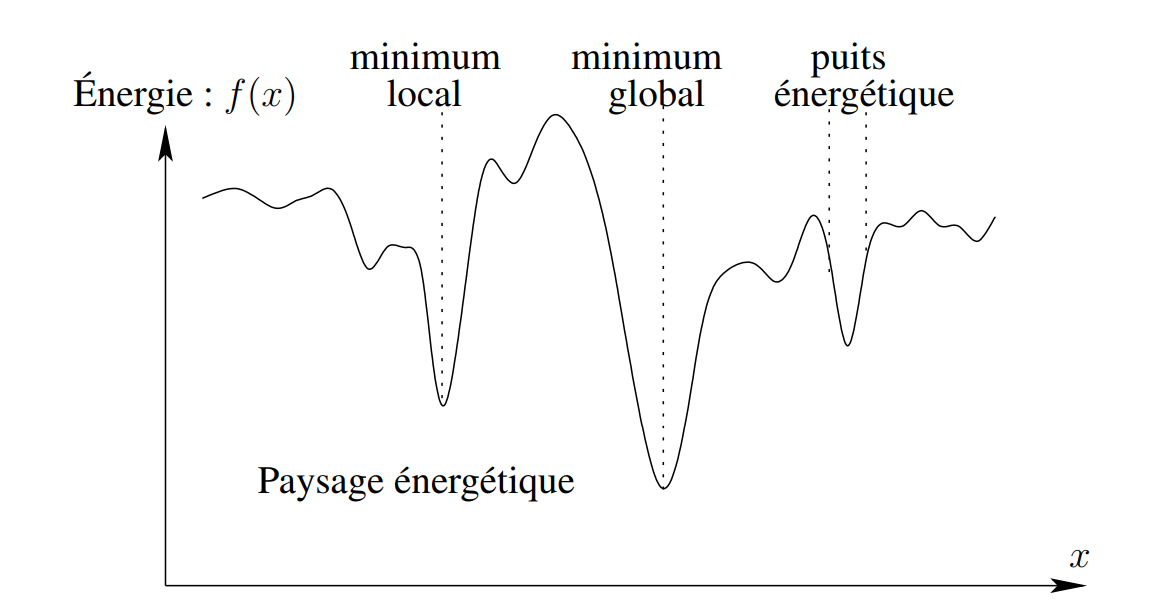
\includegraphics[height=2in]{img/Optimum_global_optimum_local.png}	
	\captionof{figure}{Paysage énergétique dans le cadre continu d’une fonction de coût pour un espace des
solutions à une dimension \citep{BICHOT2007}} \label{ogol}
\end{center}
%%%%%%%%%%%%%%%%%%%%%%%%%%%%%%%%%%%%%%%%%%%%%%%%%%%%%%%%%%%%%%%%%%%%%%%%%%%%%%%%%%%%%%%%%%%%%
%%									section.	Graphes											%
%%%%%%%%%%%%%%%%%%%%%%%%%%%%%%%%%%%%%%%%%%%%%%%%%%%%%%%%%%%%%%%%%%%%%%%%%%%%%%%%%%%%%%%%%%%%%

\section{Graphes}
Cette section rappelle quelques définitions de la théorie des graphes \citep{Francois2013}.

\begin{definition}[Graphe]
	Un graphe est un couple $G= (S, A)$, formé d'un ensemble $S$ de sommets (ou nœuds ou points) et d'un ensemble $A$ d'arêtes, d'arcs (ou lignes) qui sont associés à des sous-ensembles à deux éléments de $S$. Les sommets appartenant à une arête sont ses extrémités. Un sommet d'un graphe n'est pas nécessairement extrémité d'une arête : c'est alors un sommet isolé. La taille d'un graphe est, selon le cas, le nombre de ses sommets $\mid S \mid$ ou le nombre de ses arêtes $\mid A \mid $. Selon la nature de l'ensemble $A$, le graphe peut être orienté ou non orienté.
\end{definition}

\begin{definition}[Graphe orienté, non orienté]
	Soit un graphe $G = (S, A)$. Si $\forall (x, y) \;\in\; A$, $(y, x) \;\in\; A$, alors le graphe est dit non orienté et les éléments de $A$ sont appelés arêtes du graphe. Dans ce cas, on note indifféremment une arête : $a \;\in\; A$, $(s, s’) \;\in\; A$ avec $s$ et $s’$ dans $S$, ou encore $(s’, s)$. Dans le cas contraire, le graphe est dit orienté et les éléments de $A$ sont appelés arcs du graphe.
\end{definition}

\begin{definition}[Adjacence]
Soient un graphe $G = (S, A)$ et une arête $a = (s, s’) \;\in\; A$. On dit que les sommets $s$ et $s'$ sont les sommets adjacents (voisins) à l'arête $a$. De même, on dit que $a$ est l'arête adjacente aux sommets $s$ et $s'$.

\end{definition}

\begin{definition}[Degré d'un sommet]
Dans un graphe non orienté $G = (S, A)$, le degré d'un sommet $s \;\in\; S$ est le nombre d'arêtes auxquelles ce sommet appartient :
\begin{center}
	$deg(s) = card({(s, s') \in\; A, s' \in S})$
\end{center}
\end{definition}

\begin{definition}[Graphe Complet]
Un graphe est complet si tous ses sommets sont adjacents entre eux. Deux sommets non adjacents peuvent malgré tout avoir une certaine connections. Dans ce cas, nous parlerons de chemin.
\end{definition}

\begin{definition}[Chemin]
Un chemin dans $G = (S, A)$ de longueur $n$ est une suite de sommets $a_{1}a_{2} . . . a_{n}a_{n+1}$ reliés entre eux par des arêtes, c'est-à-dire $a_{i}a_{i+1} \;\in A$, pour $i = 1,\; 2, \; . . .,\; n$. Un cycle est un chemin fermé, C'est-à-dire que $a_{1} = a_{n+1}$.
\end{definition}

\begin{definition}[Graphe connexe]
Soit un graphe $G = (S, A)$. On dit que ce graphe est connexe si, quels que soient les sommets $s$ et $s'$ de $S$, il existe un chemin de $s$ vers $s'$. 
\end{definition}

\begin{definition}[Boucle et arête multiple]
Une arête est appelée une boucle si ses deux extrémités sont identiques. Si deux arêtes possèdent les mêmes extrémités, alors on dit que l'arête est multiple et que ces deux arêtes sont parallèles. Dans ce cas, la multiplicité d'une arête est le nombre total de ses arêtes parallèles, y compris elle-même.
\end{definition}

\begin{definition}[Graphe value ou pondéré]
Un graphe pondéré est un graphe étiqueté où chaque arêtes (arcs) est affectée d'un nombre réel positif, appelé poids de cette arête (arc).
\end{definition}

\begin{definition}[Sous-graphe]
Un sous-graphe $H = (S_H, A_H)$ d'un graphe $G = (S, A)$ est le graphe $G$ auquel des sommets et/ou des arêtes ont été enlevés, c'est-à-dire   
\begin{center}
$S_H \subseteq S$ et $A_H \subseteq A$.
\end{center}
\end{definition}

\begin{definition}[Chaîne]
	Une chaîne est une suite d'arcs partant d'un sommet $s_1$ et se terminant à un sommet $s_{n}$. Nous pouvons la définir comme suit :\begin{flushleft}
	$ G = (S, A) | S = \{s_1, s_2, ..., s_n\} \wedge A=\{a_1, a_2, ..., a_{n-1}\}\; où\; a_i = (s_i, s_i+1)\; i=1..n-1 $.
	\end{flushleft}
\end{definition}

\begin{definition}[Circuit]
Un circuit est une suite d'arcs partant et finissant au même sommet. Nous pouvons le définir comme suit: \begin{center}
$G = (S, A) | S = \{s_1, s_2, ..., s_n\} \wedge  A=\{(s_1, s_2), (s_2, s_3), ..., (s_{n-1}, s_n), (s_n, s_1)\}$
\end{center}
\end{definition}

\begin{definition}[Appariement]
Soit un graphe $G = (S, A)$. L'appariement $M$ du graphe $G$ est un ensemble d'arêtes non-adjacentes deux à deux. On dit que l'appariement est maximum lorsqu'il contient le plus grand nombre possible d'arêtes. On dit que l'appariement $M$ est maximal lorsque toute arête du graphe possède une intersection non vide avec au moins une arête de $M$.
\end{definition}

\paragraph{Remarque}
Tout appariement maximal est aussi un appariement maximum. Soit un appariement maximal $M$, si une arête quelconque de $A$ qui n'est pas dans $M$ est ajoutée à $M$, alors $M$ n'est plus un appariement de $G$. La réciproque n'est pas nécessairement exacte: soit un graphe linéaire de $4$ sommets, l'appariement composé de l'arête formée des deux sommets centraux est maximal mais pas maximum. Un graphe peut posséder plusieurs appariements maximal (et a fortiori plusieurs appariements maximum).
%%%%%%%%%%%%%%%%%%%%%%%%%%%%%%%%%%%%%%%%%%%%%%%%%%%%%%%%%%%%%%%%%%%%%%%%%%%%%%%%%%%%%%%%%%%%%
%%									section.	Partitionnement de graphe											%
%%%%%%%%%%%%%%%%%%%%%%%%%%%%%%%%%%%%%%%%%%%%%%%%%%%%%%%%%%%%%%%%%%%%%%%%%%%%%%%%%%%%%%%%%%%%%

\section{Partitionnement de graphe}
Le partitionnement de graphe est un problème NP-Complet \citep{GAREY1976}, utilisé pour résoudre un grand nombre de problèmes d'ingénierie : La conception de circuits intégrés électroniques \citep{CONG2003}, la répartition de charge pour les machines parallèles \citep{BARAT2016}, la dynamique des fluides, le calcul matriciel, la segmentation d'images \citep{GRADY2006} ou la classification d'objets \citep{DHILLON2007}.

Etant donné un graphe non-orienté $G = (S, A)$ où $S$ est l'ensemble des sommets et $A$ est l'ensemble des arêtes. Les sommets et les arêtes peuvent être pondérés. Le problème du partitionnement d'un graphe $G$ consiste à le diviser en $k$ parties disjointes. Du point de vue mathématique, on peut partitionner les sommets ou bien les arêtes. Cependant, bien que certains problèmes cherchent à partitionner les arêtes d'un graphe \citep{HOLYER1981}, on entend le plus souvent par partition d'un graphe, le partitionnement des sommets de ce graphe.

\begin{definition}[Partition des sommets d'un graphe] \citep{BichotSiarry2013}
\\Soient un graphe $G = (S,A)$ et un ensemble de $k$ sous-ensembles de $S$, noté $P_k = \{S_1, S_2, . . . ,S_n\}$. En d'autres termes, $P_k$ est dite une partition de $G$ si :
\begin{itemize}
	\item Aucun sous-ensemble de $A$ qui est élément de $P_k$ n'est vide : $\forall i\; \in \; \{1, ..., k\},\; S_i \ne \emptyset$
	\item Les sous-ensembles de $S$ qui sont éléments de $P_k$ sont disjoins deux à deux : $\forall(i, j) \in{1, ..., K}, i \ne j, S_i \cap S_j = \emptyset$
	\item L'union de tous les éléments de $P_k$  est $S$ : $U^{k}_{i=1} S_k = S$
\end{itemize}
Les éléments $S_i$ de $P_k$ sont appelés les parties de la partition.\\
Le nombre $k$ est appelé le cardinal de la partition, ou encore le nombre de parties de la partition.
Dans le cas $k = 2$, on a le problème de bissection.
\end{definition}
%%%%%%%%%%%%%%%%%%%%%%%%%%%%%%%%%%%%%%%%%%%%%%%%%%%%%%%%%%%%%%%%%%%%%%%%%%%%%%%%%%%%%%%%%%%%%
%%									section.	Approches de partitionnement										%
%%%%%%%%%%%%%%%%%%%%%%%%%%%%%%%%%%%%%%%%%%%%%%%%%%%%%%%%%%%%%%%%%%%%%%%%%%%%%%%%%%%%%%%%%%%%%

\section{Approches de partitionnement de graphes}
 Le partitionnement d'un graphe consiste à trouver une partition des sommets respectant une ou plusieurs propriétés. Ces propriétés sont de nature très diverses. On peut par exemple chercher à minimiser la capacité des arêtes externes, c'est-à-dire le nombre d'arêtes ou la somme totale des poids des arêtes reliant deux groupes.  Le problème devient difficile si on cherche à diviser le graphe en $k$ groupes de tailles équilibrées car il n'existe alors pas d'algorithme polynomial pour y répondre. Ce problème a été démontré NP-complet \citep{HYAFIL1973}, \citep{GAREY1976}

Au cours des dernières années, beaucoup d'efforts ont été consacrés au développement d'heuristiques rapides et efficaces pour ce problème. Ces heuristiques peuvent souvent gérer des graphes assez grands avec des milliers de nœuds et fournir de bonnes solutions. Pour un aperçu plus détaillé, nous nous référons à \citep{BichotSiarry2013}, \citep{BULU2016},\citep{SCHLOEGEL2000}.

Nous allons maintenant présenter les approches couramment utilisées pour résoudre le problème du partitionnement de graphes.


\subsection*{Approche exacte}
Les solutions exactes peuvent être utilisées comme des facteurs importants pour valider les heuristiques. Cependant, peux d'effort ont été faits dans le développement d'algorithmes exacts \citep{Armbruster2008}, \citep{Bonami2012}, \citep{Delling2012}, \citep{FeldmannWidmayer2015}, \citep{Ferreira1998}, \citep{Hager2013}, \citep{Kaibel2011}, \citep{Sellmann2003}, \citep{Sorensen2007}. La plupart de ces méthodes reposent sur la méthode de séparation et d'évaluation qui permet d'éviter l'exploration systématique de l'espace des solutions en éliminant les sous-arbres menant à des solutions moins bonnes qu'une solution donnée, et se diffèrent selon que l'exploration de l'arbre est réalisée en profondeur, par niveaux ou par ordre croissant des valeurs des fils non encore traités \citep{Land2010}.
Du fait de la nature NP-difficile du problème, il est clair que généralement seuls des graphes relativement petits peuvent être résolus par une approche exacte.

\subsection*{Approche spectrale}
L'approche spectrale du partitionnement de graphes repose sur le théorème spectral de l'algèbre linéaire, elle consiste à rechercher les valeurs propres de la matrice de Laplace associée au graphe $G$, ensuite l'ordonnancement de ces valeurs qui est lié à la connectivité des sommets du graphe.
Les techniques spectrales ont d'abord été utilisées par Donath et Hoffman \citep{DonathHoffman1972} et Fiedler \citep{Fiedler1973}, \citep{Fiedler1975}, et ont été améliorées par la suite par plusieurs chercheurs \citep{Boppana1987}, \citep{HendricksonLeland1995a}, \citep{Kabelikova2006}, \citep{Simon1991}.
Il a été montré que cette méthode permet d'obtenir un extremum global avec certains graphes \citep{Pothen1990}; cependant, il a aussi été mis en évidence que cette méthode est très coûteuse en terme de calculs et devient inefficaces lorsque la taille du graphe devient importante \citep{BarnardSimon1994}.

\subsection*{L'approche combinatoire} \citep{BENSETIRA2017}
Contrairement à l'approche spectrale, les travaux cités dans cette approche opèrent directement sur la structure du graphe.
L'idée générale consiste à effectuer un parcours de proche en proche d'une partie de l'ensemble $P(G)$ afin d'y trouver le meilleur candidat qui résolve le problème. En plus, un algorithme de ce type nécessite les deux données suivantes :
\begin{itemize}
\item la définition d'un voisinage dans $P(G)$;
\item l'historique des optimisations précédentes.
\end{itemize}
Le voisinage permet de définir comment l'algorithme va progresser en perturbant la solution courante $S$ : par exemple, on peut définir le voisinage de $S$ comme correspondant à un seul déplacement de sommet par l'ensemble des éléments de $P(G)$ qui peuvent être obtenus en changeant dans la partie un seul sommet de $S$.

Dans cette approche, on distingue entre les méthodes basées sur les algorithmes itératifs et les méthodes basées sur les méta-heuristiques.

\subsection*{Les algorithmes itératifs}
Les algorithmes itératifs d'optimisation fonctionnent en partant d'une partition $\prod _0 \;\in \; P(G)$ de $G$, valide et bien équilibrée, et se déplacent dans l'espace des solutions en sélectionnant le voisin le plus proche qui permet de réduire la coupe de la partition. L'algorithme s'arrête lorsqu'aucun des voisins n'est satisfaisant. Ces algorithmes convergent donc vers l'optimum local accessible depuis la partition initiale $\prod _0$ .

Bien que la convergence ne soit que locale et dépendante du point de départ dans $P(G)$, ces algorithmes sont très populaires. Les résultats produits pouvant être améliorés en effectuant plusieurs exécutions à partir de partitions initiales différentes ou en utilisant le schéma multi-niveaux qui sera présenté plus loin. Parmi les algorithmes de cette catégorie, nous pouvons citer \citep{FiducciaMattheyses1988}, \citep{Hagen1997}, \citep{KernighanLin1970}, \citep{Krishnamurthy1984}. 

Le principal défaut de ces approches itératives concerne leur vision strictement locale du problème, ce qui implique que le résultat ne peut être au mieux qu'un optimum local, fortement dépendant de la solution initiale. D'autres approches d'algorithmes d'optimisation ayant une vision plus globale peuvent être utilisées.

\subsection*{Les approches basées sur les méta-heuristiques}
 Les algorithmes génétiques, ont fait l'objet de plusieurs approches pour le problème du partitionnement de graphes \citep{BuiMoon1996}, \citep{ChevalierPellegrini2006}, \citep{ChockalingamArunkumar1992}, \citep{Soper2004}, \citep{TalbiBessiere1991}.  Le principe est d'explorer l’espace des solutions à l'aide d'une population d'individus qui vont échanger entre eux certaines de leurs caractéristiques lors d'une étape de reproduction, ceci dans le but d'obtenir de nouveaux individus combinant les qualités de leurs parents tout en essayant d'en diminuer les défauts. Pour un aperçu général des algorithmes génétiques abordant le problème du partitionnement de graphe, nous renvoyons le lecteur à l'article de \citep{Kim2011}.

Les principales difficultés d'application de ces algorithmes tiennent d'une part à la multitude de paramètres qu'il faut régler en fonction de la nature du problème, d'autre part à leurs coûts en mémoire et en temps : La taille de la population est liée à celle du problème et le temps est dépendant du nombre de générations qui est lié à la taille de la population.

Les méthodes de colonies de fourmis consistent à imiter le comportement des fourmis qui exploitent une méthode de résolution collective. En effet, les fourmis utilisent des phéromones pour marquer les différents chemins empruntés et la concentration de ces marqueurs chimiques est
d'autant plus importante que la fréquence d'utilisation est importante. Pour le k-partitionnement, l'idée est donc d'utiliser $k$ colonies de fourmis dont le but est d'accumuler la nourriture qui est distribuée sur les sommets du graphe, l'exploration est guidée par la répartition des colonies, de la nourriture et par les décisions des fourmis \citep{Korosec2004}, \citep{LanghamGrant1999}, \citep{Jovanovic2016}.

D'autres méta-heuristiques, comme la recherche tabou \citep{BattitiBertossi1999}, le recuit simulé \citep{Bichot2004}, \citep{Johnson1989}, \citep{Williams1991}, les algorithmes de gradients aléatoires adaptatifs (GRASP) \citep{AreibiYang2004}, les méthodes de diffusion stochastique \citep{TaoZhao1993}, \citep{Wan2005}, ont été appliquées avec plus ou moins de succès au partitionnement de graphe.

On peut aussi citer les travaux basés sur la méthode de percolation \citep{MeyerhenkeSchamberger2006}, \citep{Pellegrini2007} qui s'inspire du principe de l'écoulement d'un fluide à travers un solide poreux, et la méthode de fusion-fission \citep{Bichot2007} qui s'inspire de la physique nucléaire et plus particulièrement des fusions et fissions d'atomes.
L'efficacité des méthodes combinatoires est étroitement liée à la taille de l'espace de recherche, les heuristiques calculent un partitionnement acceptable en un temps polynomial.


\subsection*{L'approche multi-niveaux}
La méthode multi-niveaux, introduite par \citep{BarnardSimon1994}, \citep{HendricksonLeland1995b}, \citep{VanDriesscheRoose1994}, permet de réduire la taille du graphe ainsi que celle de l'espace de recherche tout en procurant l'accès à une vision globale pour les algorithmes
combinatoires. L'idée principale est de travailler sur un graphe réduit ayant les mêmes propriétés topologiques que le graphe initial (regrouper les sommets ensemble pour traiter de groupes de sommets plutôt que de sommets indépendants).
Pour ce faire, le schéma multi-niveaux comporte trois étapes (Figure \ref{pmn}) :
\begin{enumerate}
	\item  L'étape de contraction, durant laquelle on applique récursivement une fonction de contraction afin de diminuer la taille du graphe;
	\item  L'étape de partitionnement initial, où l'on applique une heuristique sur le plus petit graphe;
	\item  L'étape d'affinage, durant laquelle la partition initiale est projetée et raffinée sur les graphes de plus en plus gros jusqu'au graphe initial.
\end{enumerate}
  
	\begin{center}
		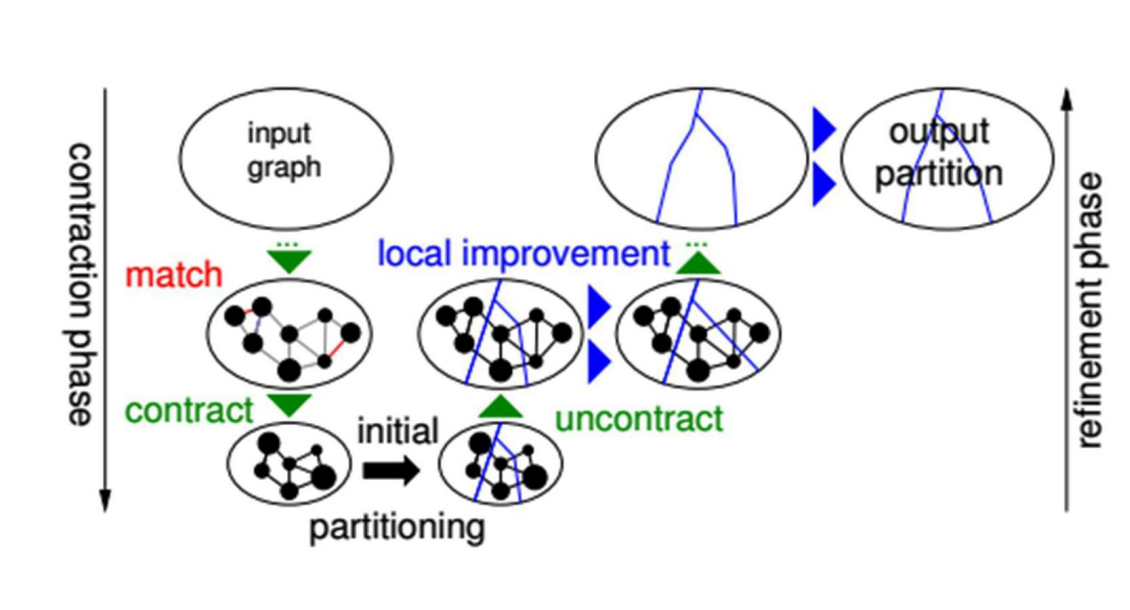
\includegraphics[height=2in]{img/multiniveaupartitionnement.PNG}		
		\captionof{figure}{ L'approche multi-niveau du partitionnement de graphe, \citep{SandersSchulz2011}} \label{pmn}
	\end{center}
Dés lors, plusieurs améliorations ont été proposées \citep{Aurora2007}, \citep{ChevalierSafro2009}, \citep{KalayciBattiti2018}, \citep{Karypis2003}, \citep{KarypisKumar1998}, \citep{Monien2000}, \citep{Pellegrini1995}, \citep{Pope2016}, \citep{Predari2017}, \citep{Safro2015}, \citep{SandersSchulz2011}, \citep{Talu2017}.


\subsection*{La parallélisation du partitionnement de graphes}
Des tentatives de parallélisation des algorithmes de partitionnement de graphes ont vu le jour. On peut citer ParMeTiS \citep{Karypis2011}, ParJostle \citep{Walshaw2012}, PT-Scotch \citep{ChevalierPellegrini2008}, et Parkway \citep{TrifunovicKnottenbelt2004} pour le partitionnement d'hyper-graphes. Tous ces outils utilisent un schéma multi-niveaux parallèle.

Des approches qui combinent les différentes méthodes présentées ci dessus ont été proposées, \citep{Chan2016}, \citep{LaSalleKarypis2013}, \citep{LaSalleKarypis2015}, \citep{LengYu2007}, \citep{Rahimian2013}, \citep{SandersSchulz2012}, \citep{Tashkova2011}.



%%%%%%%%%%%%%%%%%%%%%%%%%%%%%%%%%%%%%%%%%%%%%%%%%%%%%%%%%%%%%%%%%%%%%%%%%%%%%%%%%%%%%%%%%%%%%
%%									section.	Distribution de graphes											%
%%%%%%%%%%%%%%%%%%%%%%%%%%%%%%%%%%%%%%%%%%%%%%%%%%%%%%%%%%%%%%%%%%%%%%%%%%%%%%%%%%%%%%%%%%%%%

\section{Distribution de graphes}
Le contexte général de notre projet de fin d'étude est la vérification formelle des systèmes. Les systèmes à vérifier sont représentés par des modèles de spécification formels, qui génèrent sous une sémantique formelle des espaces d'états. Un espace d'états peut être considéré comme un graphe. Dans ce contexte particulier, on parle de distribution de graphes (espaces d'états), et non pas de partitionnement de graphe. Les différences principales entre eux résident dans le fait que:
\begin{itemize}
\item  Le partitionnement des graphes opèrent sur des graphes simples non orientés et pondérés. Alors que dans notre contexte, les graphes sont orientés, non pondérés, et contiennent dans la plupart des cas des cycles.
\item  En générale, les applications qui utilisent le partitionnement des graphes supposent l'existence préalable du graphe. Tandis que les espaces des états sont construits au moment de leurs distribution.
\item La distribution d'un graphe n'interdit pas la duplication de certains de ses états (sommets) sur plusieurs parties distribuées du graphes.
\end{itemize}

\subsection*{L'espace d'états distribué}{
Dans cette section, nous définissons la structure d'un espace d'états distribué qui se compose de sous-graphes localisés dans les différentes machines disponibles sur le réseau. 


Un espace d'état est une structure relationnelle qui représente le comportement d'un système (programme, protocole, réseau social, ...). Il représente tous les états possibles du système et les transitions entre eux. Un espace d'états est un graphe orienté $G = (S, A)$ avec un ensemble de sommets $S$, un ensemble d'arcs $A$.}


\begin{definition}
Soit $M =\{M_K\}_{K=1..N}$ $N$ machines. Un espace d'états distribué, noté $DiG$, est un graphe avec une fonction de distribution $f^k$. $DiG = (G; f^k )_{ k=1..N}$ , tel que : $G = (S, A)$ : est un graphe dirigé.
$f^k : G \Rightarrow G_k$ : est une application de G dans G k , tel que \\$G_k = (S_k , A_k )$ : $\{G_K \}_{1<k<N}$ est un ensemble de sous-ensembles appelés fragments $G_k $, tel que :\\ $U^{N}_{k=1} S_k = S\; et\; U^{N}_{k=1}A_k = A$
\end{definition}

\begin{definition} \citep{BENSETIRA2017}\\
Un fragment $G_k$ est définit par $G_k = (S_k , A_k )$ de tel sorte que :
\begin{itemize}
\item $S_k\subseteq S$ est un fragment des états de $S$ dans la machine $M_k$ tel que :
	\begin{itemize}
	\item  Aucun élément de $S_k$ n'est vide : $\forall \;k \in \;1, ..., N,\; S_k \ne \emptyset$
	\item L'union de tous les éléments de $S_k$ est égale à $S$ : $U^{N}_ {k=1} S_k = S$
	\end{itemize}
\item $A_k = A^{L}_{K}\cap A^{K}_{R}$ tel que  $A^{L}_{K} \cap A^{K}_{R}= \emptyset$ : l'ensemble des transitions internes et externes avec :
	\begin{itemize}
	\item  $A^{L}_{K}\subseteq S_K \times S_K$ est l'ensemble des transitions entre les états qui appartient à la même machine $M_k$ (transitions locales ou internes)
	\item  $A^{R}_{K}\subseteq S_K \times (S/S_K ) \cup (S/S_K ) \times S_K = (s, s')$, tel que soit $(s \in S_K et s' \neq S_K ) ou(s \neq S_K et s'
\in S_K )$ : est l'ensemble des transitions dont les origines se trouvent dans des machines locales et les états cibles (destination) sont dans des machines distantes (transitions externes) et inversement.
	\end{itemize}
	
\end{itemize}
Le nombre $k$ est appelé la cardinalité du fragment.
\end{definition}

La Figure \ref{eed}(a) représente un espace d'états, et une distribution possible de cet espace sur un réseau de trois machines (Figure \ref{eed}(b)). Les transitions internes sont marquées avec des lignes continues, et les transitions externes sont marquées avec des lignes en pointillés.

\begin{center}
		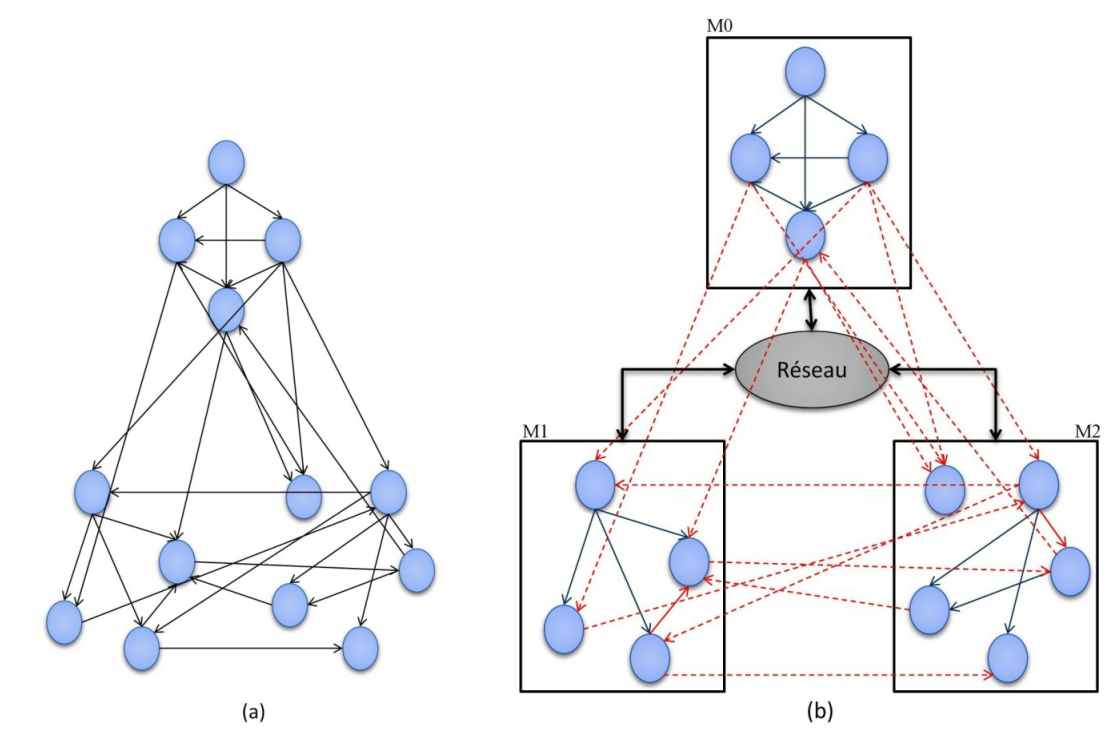
\includegraphics[height=3in]{img/eed.PNG}		
		\captionof{figure}{Un espace d’état et sa distribution sur un cluster de 3 machines, \citep{BENSETIRA2017}} \label{eed}
\end{center}

\subsection*{Approche de distribution des espaces d'états}
\paragraph{Distribution basée sur des fonctions}
 La plupart des solutions proposées pour la distribution des espaces d'états reposent sur l'utilisation d'une fonction de distribution qu'elle soit statique \citep{Garavel2013}ou dynamique \citep{Allmaier1997}, basée sur la structure de formalisme de spécification utilisé \citep{Ciardo1998}, \citep{BlomOrzan2005} ou guidée par des heuristiques \citep{Rodrigues2006}.
 \paragraph{Distribution basée sur la coloration}
 Cette approche consiste à introduire le concept de coloration et la relation de dominance dans les graphes pour trouver la bonne distribution des graphes L'approche proposée dans \citep{Guidoum2013} est basée sur le concept de la coloration forte stricte des graphes \citep{Bouzenada2012}. L'approche proposée est divisée en deux parties : un processus d'initialisation et un processus d'optimisation. Dans la première étape, les auteurs utilisent l'algorithme de coloration \citep{Bouzenada2012} qui assure la propriété de dominance. Les sorties de ce dernier (le nombre de couleurs dominées, ensemble de sommets colorés) sont exploitées pour répartir initialement le graphe et obtenir des parties disjointes. Ensuite le processus d'optimisation est utilisé pour trouver la bonne distribution.
 
 \paragraph{Distribution basé sur les métaheuristiques}
Récemment une nouvelle alternative de distribution des espaces d'états a été investiguée. Les approches proposées dans cette classe se basent sur l'utilisation des méthodes d'optimisation combinatoire, qui ont montré leur efficacité de résolution des problèmes dans différents domaines d'application.
 \\\\ 
Saidouni et al. \citep{Saidouni2012} proposent un nouvel algorithme de distribution inspiré de l'algorithme d'optimisation par essaims de particules. Les auteurs ont pu montrer comment les composants de la métaheuristique PSO comme le voisinage, les particules, et leurs vitesses et direction peuvent être adaptés pour la distribution des graphes sur une plateforme de N machines. L'approche fournit un bon équilibrage de charge et une réduction des connexions externes dans le réseau. Cependant, cette approche souffre du problème des états redondants.
\\\\
Une autre approche a été développée dans  \citep{TabibSaidouni2016},  \citep{Tabib2017}, où les auteurs ont proposé un algorithme génétique basé sur la loi gravitationnelle de Newton pour la distribution de graphes. La particularité de cette approche est que les espaces d'états sont codés par les diagrammes de décision binaires, et l'utilisation d'un modèle génétique en ilot qui repose sur l'exécution parallèle de plusieurs machines qui contiennent des populations de même taille avec la migration de leur m meilleurs individus chaque $n$ cycles.
\\\\
Saidouni et Bensetira \citep{BENSETIRA2017}, proposent un nouvel algorithme de distribution de l'espace d'états basée sur le comportement des systèmes. La particularité de cette approche est que les états sont analysés, ensuite, selon les informations pertinentes sur les états et leurs connexions (transitions internes et externes), ils sont redistribués selon une certaines heuristiques afin d'optimiser les performances
du système. Cela se fait en définissant une bonne localité d'un état comme celle qui optimise à la fois l'équilibre de la charge de travail et la quantité de communication entre les machines engendrés par l'exécution de l'application opérant sur l'espace d'états distribués.
\section{Conclusion}{
Dans ce chapitre, nous avons introduit quelques notions sur les graphes, ensuite nous avons donné un bref aperçu du travail qui a été fait sur le partitionnement et la distribution des graphes. Il nous est alors possible de développer de nouveaux algorithmes de distribution de graphe en exploitant le model cheching et les méthodes  d'optimisation combinatoire.
}		
		%%%%%%%%%%%%%%%%%%%%%%%%%%%%%%%%%%%%%%%%%%%%%%%%%%%%%%%%%%%%%%%%%%%%%%%%%%%%%%%%%%%%%%%%%%%%%
%%									Chapitre Approche de partitionnement et de distribution des graphes
%%%%%%%%%%%%%%%%%%%%%%%%%%%%%%%%%%%%%%%%%%%%%%%%%%%%%%%%%%%%%%%%%%%%%%%%%%%%%%%%%%%%%%%%%%%%%
\chapter{  Model Checking}
	\minitoc
	\newpage

%%%%%%%%%%%%%%%%%%%%%%%%%%%%%%%%%%%%%%%%%%%%%%%%%%%%%%%%%%%%%%%%%%%%%%%%%%%%%%%%%%%%%%%%%%%%%
\section{Introduction} 
De nos jours, la vie des êtres humains dépend largement des systèmes informatiques qui remplissent des fonctions de plus en plus critiques. Ceci à augmenter la difficulté d'assurer le bon fonctionnement de ces systèmes afin d'éviter des conséquences qui peuvent s'avérer fatales, coûteuses et dramatiques \citep{Huckle2015}, \citep{Kanaracus2012}. Dès lors, il faut fournir des techniques de vérification et de validation efficaces et performantes qui garantissent la sûreté de fonctionnement de ces systèmes critiques et qui prennent en charge leurs complexités croissantes \citep{Ferrari1978}.

Les méthodes formelles apportent une solution à ce problème, car elles permettent de définir des modèles mathématiques décrivant  rigoureusement le comportement des systèmes. Elles les décrivent principalement à l'aide de langages formels adaptés et définis avec précision au niveau de la syntaxe et de la sémantique. Une fois décrit, elles peuvent prouver la correction du modèle en utilisant des méthodes de vérification formelle. La vérification consiste alors à s'assurer que l'ensemble des fonctionnements du système développé satisfait tous les besoins \citep{ClarkeWing1996}, \citep{Dsilva2008}.
 
Le model checking est une forme de vérification formelle des systèmes \citep{Cheng2006}, \citep{Wang2004}. Son principe est de vérifier que le modèle représentant le système, respecte bien les propriétés que l'on attend de lui, d'où le terme model checking. Les systèmes sont spécifiés par des formalismes tels que les automates temporisés \citep{AlurDill1994}, et les propriétés sont exprimées par des assertions dans une logique, par exemple la logique temporelle \citep{BenAri1983}. Bien que cette technique soit restreinte à des systèmes ayant un nombre fini d'états, elle permet une détection rapide et économique des erreurs dans des systèmes complexes. Parmi les outils les plus connus, on peut citer UPPAAL, DiVine, CADP, Murphi, Roméo, SPIN \citep{Behrmann2004}, \citep{Barnat2010}, \citep{Garavel2013}, \citep{Dill1996}, \citep{Lime2009}, \citep{Holzmann2003}.

Les réseaux de Petri sont des outils à la fois graphiques et mathématiques permettant de modéliser le comportement dynamique des systèmes à  évènements discrets. Leur représentation graphique permet de visualiser d'une manière naturelle le parallélisme, la synchronisation, le partage de ressources, les choix (conflits), etc. Leur représentation mathématique permet d'analyser le modèle pour étudier ses propriétés    et de les comparer avec le comportement du système réel. L'une des approches de vérification d'un réseau Petri consiste à générer son graphe de marquage dont les sommets représentent les états dans lesquels le système peut se trouver, et dont les arcs représentent les transitions faisant passer le système d'un état à un autre. Après la génération, le graphe de marquage peut être vu comme un système de transitions étiquetées \citep{Arn92}. Le système de transitions étiquetées, ainsi généré, est utilisé pour la vérification des propriétés du système spécifié par le réseau (model checking, bissimilarité, test de conformité, etc. \citep{CES86}, \citep{FM}, \citep{CH93}). Cependant, le modèle des systèmes de transitions étiquetées fait abstraction quant à l'exécution parallèle des transitions.


Nous nous intéressons dans ce chapitre, au réseaux de Petri et au model checking distribuée. Nous présentons dans un premier lieu  les réseaux de Petri, puis les systèmes de transitions étiquetées et aussi la structure de Kripke. Enfin, on termine avec le model checking distribué.

\section{Réseaux de Petri}
Les Réseaux de Petri (abréviation  RdP) ont été introduits par le mathématicien Allemand Carl Adam Petri dans sa thèse \citep{Carl1962}, d'où leur appellation Réseaux de Petri (ou Petri Nets en anglais). Ces derniers méritent bien leur  appellation  car  la  thèse de C.A Petri a présenté un certain nombre d'idées fondamentales du modèle. Mais la théorie des RdP en sa totalité, telle que nous la connaissons actuellement est le résultat de fusionnement et de contribution directe ou indirecte des travaux de plusieurs  chercheurs de différentes universités et de différents laboratoires \citep{Robert2007}.

Les réseaux de Petri sont des outils à la fois graphiques et mathématiques permettant de modéliser le comportement dynamique des systèmes à  évènements discrets et d'évolutions simultanées. Leur représentation graphique permet de visualiser d'une manière naturelle le parallélisme, la synchronisation, le partage de ressources, les choix (conflits), etc. Leur représentation mathématique permet d'analyser le modèle pour étudier ses propriétés et de les comparer avec le comportement du système réel.

Cette section présente les notions fondamentales des réseaux de Petri.

\begin{definition}[Informelle]
Un réseau de Petri est un graphe biparti dont les sommets sont répartis selon deux types,  les places et les transitions. Ce graphe est constitué de telle sorte que les arcs du graphe ne peuvent relier que des places aux transitions ou des transitions aux places. Les places sont représentées par des cercles, alors que les transitions sont représentées par des traits ou des rectangles (Figure \ref{rdp}). Les places servent  à représenter les états du  système modélisé, tandis que les  transitions  représentent les changements d'état ou les événements \citep{SaidounicoursRdp2017}.

\begin{center}
	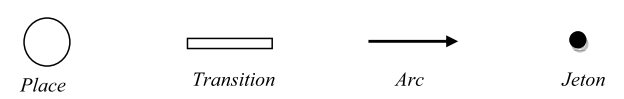
\includegraphics[scale=0.5]{img/rdp.PNG}
	\captionof{figure}{Représentation graphique des éléments d'un RdP} \label{rdp}
\end{center}


 Chaque place peut contenir un nombre entier de jetons. Les jetons modélisent souvent l'état d'une ressource (nombre d'instances, occupée ou non, ...). Un jeton est représenté par un petit cercle noir. Pour des commodités de présentation on met à l'intérieur d'une place le nombre de jetons présents (Figure \ref{place}). 
 
 \begin{center}
	
\includegraphics[scale=0.5]{img/place.PNG}
	\captionof{figure}{ Marquage d’une place } \label{place}
 \end{center}

 À  chaque arc est associé un nombre entier strictement positif appelé poids de l'arc. Lorsque le poids n'est pas signalé, il est égal à $"1"$  par défaut. Le RdP dont tous ses arcs sont de poids "1" est appelé RdP ordinaire (Figure \ref{rdpo}). Dans le cas o\`{u} les arcs peuvent avoir des poids supérieurs à $"1"$, il s'agit de RdP généralité (Figure \ref{rdpg}).
 
 \begin{center}
	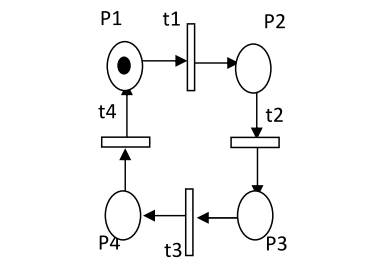
\includegraphics[scale=0.5]{img/rdp1.PNG}
	\captionof{figure}{RdP ordinaire} \label{rdpo}
 \end{center}
 
 \begin{center}
	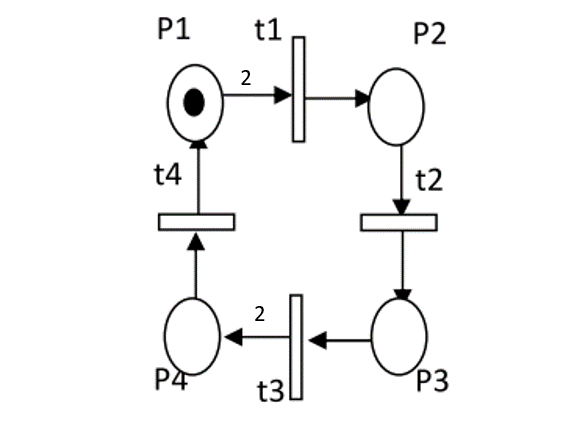
\includegraphics[scale=0.5]{img/rdpg.PNG}
	\captionof{figure}{RdP généralité} \label{rdpg}
 \end{center}
\end{definition}

\begin{definition}[Formelle]\citep{Murata1989}\\
Formellement un RDP est un quintuplet, $R= (P, T, Pre,Post , M_0 )$ tel que:
\begin{itemize}
	\item P : L'ensemble des places;
	\item T : L'ensemble des transitions;
	\item Pre : $(P  \times T)\rightarrow IN$, est l'application d'incidence avant, correspondant aux arcs directs reliant les
places aux transitions;
	\item Post : $(T  \times P)\rightarrow IN$,est l'application d'incidence arrière, correspondant aux arcs directs reliant
les transitions aux places;
	\item La matrice incidence du réseau est $C=Post-Pre$;
	\item $M_0$ : Le marquage initial (état initial). 
\end{itemize} 
\paragraph{Notation}
\begin{itemize}
	\item °t : L'ensemble des places d'entrée de la transition t;
	\item t° : L'ensemble des places de sortie  de la transition t;
	\item °p : L'ensemble des transitions  d'entrée de la place p; 
	\item P° : L'ensemble de transitions de sortie de la place p;  
\end{itemize}
Le RdP de la Figure \ref{rdp1} décrit le cycle des quatre saisons. Les places représentent les saisons,   $p_1$; le printemps, $p_2$; l'été,   $p_3$: l'automne et $p_4$: l'hiver. Les transitions représentent les changements de saisons, $t_1$; le début d'été, $t_2$; le début d'automne, $t_3$: le début d'hiver et $t_4$: le début du printemps. Le jeton dans la place $p_1$ indique que la saison à l'instant initial est le printemps. Ce scénario est modélisé comme suit:\\ 
$P= \{p 1 , p 2 , p 3 , p 4 \}$,\\ 
$T= \{t 1 , t 2 , t 3 , t 4 \}$, \\  
$Pre(p_1 ,t_1 )=1,\;\; 
Post(t_1 ,p_2 )=1,\;\; 
Pre(p_2 ,t_2 )=1,\;\; 
Post(t_2 ,p_3 )=1,\;\; 
Pre(p_3 ,t_3 )=1,\\ 
Post(t_3 ,p_4 )=1,\;\; 
Pre(p_4 ,t_4 )=1,\;\; 
Post(t_4 ,p_1 )=1$ ,  \\
$^{\circ}t_1=\{p_1 \},\;\; 
t_1^{\circ} =\{p_2 \},\;\; 
^{\circ}t_2=\{p_2 \},\;\; 
t_2^{\circ} =\{p_3 \},\;\; 
^{\circ}t_3=\{p_3 \},\;\; 
t_3^{\circ}=\{p_4 \},\;\; 
^{\circ}t_4=\{p_4 \},\;\; 
t_4^{\circ} =\{p_1 \}$,\\
$^{\circ}p_1= \{t_4 \},\;\; 
p_1^{\circ} = \{t_1 \},\;\; 
^{\circ}p_2= \{t_1 \},\;\; 
p_2^{\circ} =\{t_2 \},\;\; 
^{\circ}p_3= \{t_2 \},\;\; 
p_3^{\circ} = \{t_3 \},\;\; 
^{\circ}p_4= \{t_3 \},\;\; 
p_4^{\circ} = \{t_4 \}$.
 \begin{center}
	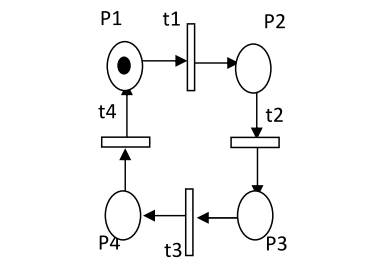
\includegraphics[scale=0.5]{img/rdp1.PNG}
	\captionof{figure}{Réseaux de Petri de quatre saisons} \label{rdp1}
 \end{center}
\end{definition}

\begin{definition}[Sensibilisation d'une transition]
Une transition $t$ est dite sensibilisée (validée, franchissable ou tirable) si chacune des places d'entrée $p$ contient un nombre de jetons supérieur ou égal au poids de l'arc reliant $p$ à $t$ \citep{SaidounicoursRdp2017}.  
$$ \forall p \in P, M(p) \geq  Pre (p, t) $$
\end{definition}

\begin{definition}[Franchissement d'une transition]
Le franchissement d'une transition $t$ sensibilisée retire de chacune de ses places d'entrée $p$ un nombre de jetons égal au poids de l'arc reliant $p$ à $t$ $(Pre (p, t))$ et dépose sur chacune de ses places de sortie p un nombre de jetons égal au poids de l'arc reliant $t$ à $p$ $(Post (p, t))$ \citep{SaidounicoursRdp2017}. Le franchissement d'une transition dans un marquage $M$ donne un nouveau marquage $M'$ défini par:
$$ \forall p \in P : M'(p)= M(p)+ C(p,t) $$

La Figure \ref{atom} illustre la réaction chimique $(2H_{2} + O_{2} \rightarrow 2H_{2}O)$ et le changement de marquage après le franchissement de la transition $t$. Avant le franchissement $M_ 0 =[2\; 2\; 0]$, après le franchissement $M_1 =[0\; 1\; 2]$. Les places sont ordonnées dans ce vecteur comme suit: $H_2 , O_2 , H_2 O$, le marquage de la place $H_2$ est noté par $M(H_2 )$. $M_0 (H_2 )$ est le marquage initial de la place $H_2$. Dans cet exemple $M_0 (H_2 ) =2$. 

\begin{center}
	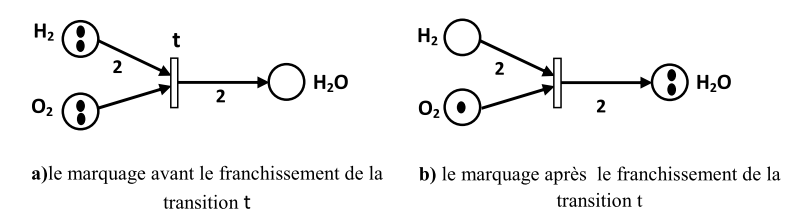
\includegraphics[scale=0.5]{img/H2O.PNG}
	\captionof{figure}{La composition d'eau $(2H_{2} + O_{2} \rightarrow 2H_{2}O)$ sous forme d'un RdP} \label{atom}
 \end{center}
\end{definition}\paragraph{Remarque }
 Lorsqu'une transition est validée, cela n'implique pas qu'elle sera immédiatement franchie; cela ne représente qu'une possibilité de franchissement, dans un  RdP, même si plusieurs transitions sont validées par un même marquage une et seulement une transition peut être franchie.
 
 
\begin{definition}[Graphe des Marquages]
Le graphe des marquages du réseau $G(R, M_0 )$ est défini par un graphe orienté dont les sommets sont étiquetés par les marquages des états accessibles $Acc(R, M_0 )$ et dont les arcs sont étiquetés par des transitions de $L(R, M_0 )$.
Un marquage $M_i$  est accessible (atteignable) à partir de $M_0$ , s'il existe une séquence $s$ de franchissement de transitions qui permet d'atteindre $M_i$  à partir de $M_0$. On note: $M_0  [s > M_i  $


La construction du graphe des marquages $G$ est faite comme suit \citep{SaidounicoursRdp2017}:
\begin{itemize}
	\item Pour chaque marquage $M$ obtenu à partir de $M_0$, trouver toutes les transitions franchissables $t_i$;
	\item Pour chaque transition $t_i$, trouver son marquage $M’$;
	\item Construire le nouveau nœud s'il est différent de ceux déjà obtenus, puis ajouter l'arc correspondant au marquage actuel vers le prochain;
	\item Continuer l'exploration tant que des marquages et des transitions n'ont pas été encore considérés.
\end{itemize}
La Figure \ref{gm1} illustre le graphe des marquages obtenue à partir du RdP de la Figure \ref{atom}.
\begin{center}
	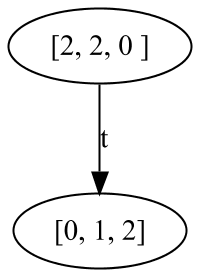
\includegraphics[scale=0.4]{img/gm1.png}
	\captionof{figure}{Graphe des marquages de $(2H_{2} + O_{2} \rightarrow 2H_{2}O)$} \label{gm1}
 \end{center}
\end{definition}

\begin{definition}[Système de transitions étiquetées]
Un système de transitions étiquetées appelé aussi $STE$ est un graphe orienté dont les sommets et les arcs de ce graphe orienté sont appelés respectivement états et transitions. Ces états et transitions sont associés avec une chaîne de caractères de manière à pouvoir les  distinguer entre eux.  Ces chaînes de caractères s'appellent \emph{noms} lorsqu'elles sont associées aux états, et étiquettes lorsqu'elles sont associées aux transitions .


Formellement un système de transitions étiquetées  est un quadruplet $\; STE = (S, Act, \delta, s_0)$ \citep{Saidouni2012}:
\begin{itemize}
	\item\textbf{S} est un ensemble (dénombrable) d'états;
	\item \textbf{Act}  est un ensemble (dénombrable) d'actions dites observables; 
 	\item  $\delta\subseteq \; S \times (Act \cup \{i\})$ : est l'ensemble des transitions, $i \notin Act$ est appelée action invisible (interne ou non-observable). Un élément $(x, a, y) \in \delta $ sera aussi noté par $x \stackrel{a}{\rightarrow}y$.
 	\item $s_0$ $\in\; S$ est l'état initial de $STE$. 
\end{itemize}

La Figure \ref{ste} illustre le STE du graphe de marquage de la Figure \ref{gm1}.
\begin{center}
	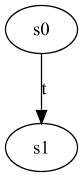
\includegraphics[scale=0.4]{img/ste.png}
	\captionof{figure}{STE de $(2H_{2} + O_{2} \rightarrow 2H_{2}O)$} \label{ste}
 \end{center}
\end{definition}

\begin{definition}[Structure de Kripke]
Une Structure de Kripke est un graphe orienté dont les nœuds représentent les états accessibles du système et dont les arcs représentent les transitions entre les états. Une fonction d'étiquetage fait correspondre à chaque état un ensemble de propositions logiques vraies dans cet état \citep{Kripke1963}.

Formellement une structure de Kripke est un 4-uplet ${\displaystyle M=(S,I,R,L)}$ \citep{Edmund1999}:
\begin{itemize}
	\item \textbf{S} est un ensemble fini d'états;
	\item \textbf{I} $\subseteq$ \textbf{S} est un ensemble d'états initiaux;
	\item \textbf{R} $\subseteq$ \textbf{S}$\times$\textbf{S}  est une relation de transition qui vérifie: pour tout ${\displaystyle s\in S}$, il existe ${\displaystyle s'\in S} $ tel que ${\displaystyle (s,s')\in R}$;
	
Soit ${\displaystyle AP}$ un ensemble de propositions atomiques, c'est-à-dire des expressions booléennes portant sur des variables, des constantes et des prédicats. On note ${\displaystyle 2^{AP}} $ l'ensemble des parties de ${\displaystyle AP}$.
	\item \textbf{L: S} $\rightarrow 2^{AP}$ est une fonction d'étiquetage(ou d'interprétation) définit pour chaque état ${\displaystyle s\in S}$ l'ensemble ${\displaystyle L(s)}$ de toutes les propositions atomiques qui sont valides dans cet état.
\end{itemize}

\paragraph{Remarque}
La condition associée à la relation de transition ${\displaystyle R}$ spécifie que chaque état doit avoir un successeur dans ${\displaystyle R}$, ce qui implique que l'on peut toujours construire un chemin infini dans la structure de Kripke. Cette propriété est importante lorsque l'on traite des systèmes réactifs\citep{Klaus2004}. Pour modéliser un interblocage dans une structure de Kripke, il suffit de faire boucler l'état d'interblocage sur lui-même.


Un chemin dans la structure ${\displaystyle M}$ est une suite ${\displaystyle c=s_{1},s_{2},s_{3},\ldots }$ d'états tels que ${\displaystyle (s_{i},s_{i+1})\in R}$ pour tout ${\displaystyle i}$. L'étiquette du chemin est la suite d'ensembles ${\displaystyle w=L(s_{1}),L(s_{2}),L(s_{3}),\ldots }$,$\ldots$ qui peut être vu comme un mot infini sur l'alphabet ${\displaystyle 2^{AP}}$.

\end{definition}

La Figure \ref{stkrdp} représente une structure de Kripke dont l'ensemble de propositions atomiques est ${\displaystyle AP=\{p,q\}}$. Ici ${\displaystyle p}$   et ${\displaystyle q}$  sont des propriétés booléennes quelconques. L'état \emph{$s_1$} contient les deux propositions, les états \emph{$s_2$} et \emph{$s_3$} respectivement ${\displaystyle q}$  et ${\displaystyle p}$. L'automate admet le chemin ${\displaystyle c=s_1,s_2,s_1,s_2,s_3,s_3,s_3,\ldots }$, et le mot ${\displaystyle w=\{p,q\},q,\{p,q\},q,p,p,p,\ldots }$ est la suite des étiquettes associées.

\begin{center}
	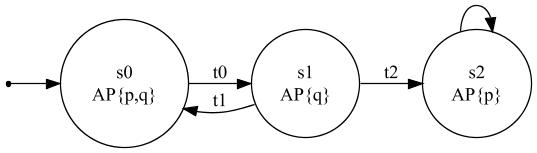
\includegraphics[scale=0.4]{img/stk.png}
	\captionof{figure}{Une structure de Kripke à trois états, avec deux propositions} \label{stkrdp}
 \end{center}
 
 
La distribution de l'espace d'états entraine la fragmentation de la structure de Kripke. Les structures partielles de Kripke modélisent des espaces d'états incomplets à parties inconnues (états border). L'évaluation des formules logiques temporelles sur les structures partielles de Kripke repose donc sur des interprétations à trois valeurs; la valeur de vérité supplémentaire \textbf{$\perp$ }  signifie « inconnu si la propriété est vraie ou fausse ».\\
Formellement une structure partielle de Kripke est un 4-uplet \\${\displaystyle F_M(T) = (S_T , I_T , R_T , L_T )}$ \citep{depriester2011bouneb}:
\begin{itemize}
	\item $T \subseteq S $;
	\item \textbf{$S_T$}  est une sous ensemble d'états fini de l'espace d'états S;
	\item \textbf{$R_T$} $\subseteq$ \textbf{$S_T$}$\times$\textbf{$S_T$}  est une relation de transition qui vérifie: pour tout ${\displaystyle s\in T}$, il existe ${\displaystyle s'\in S_T} $ tel que ${\displaystyle (s,s')\in R}$;
	\item $I_T$ est un ensemble fini d'états qui vérifie: pour tout $ s \in S_T $ tel que $ s \in I \}$;
	\item $ L_T$ : $S_T \times P \rightarrow \{ false, \perp , true \} $.
\end{itemize}

La Figure \ref{stkrdpd} représente des structures partielles de Kripke reparties sur trois machines, dont l'ensemble de propositions atomiques est ${\displaystyle AP=\{a,b,c\}}$. La répartition des états est faite comme suit:  
\begin{itemize}
 \item Sur la machine $M_1$ la structure partielle renferme deux états à parties complètes $s_0$ et $s_1$, et deux états à parties incomplètes $s_2$ et $s_4$;
 \item Sur la machine $M_2$ la structure partielle renferme un état à partie complète $s_4$, et un état à partie incomplète $s_5$;
 \item Sur la machine $M_3$ la structure partielle renferme deux  états à parties complètes $s_2$ et $s_5$, et deux états à parties incomplètes $s_1$ et $s_4$
 \end{itemize}

\begin{center}
	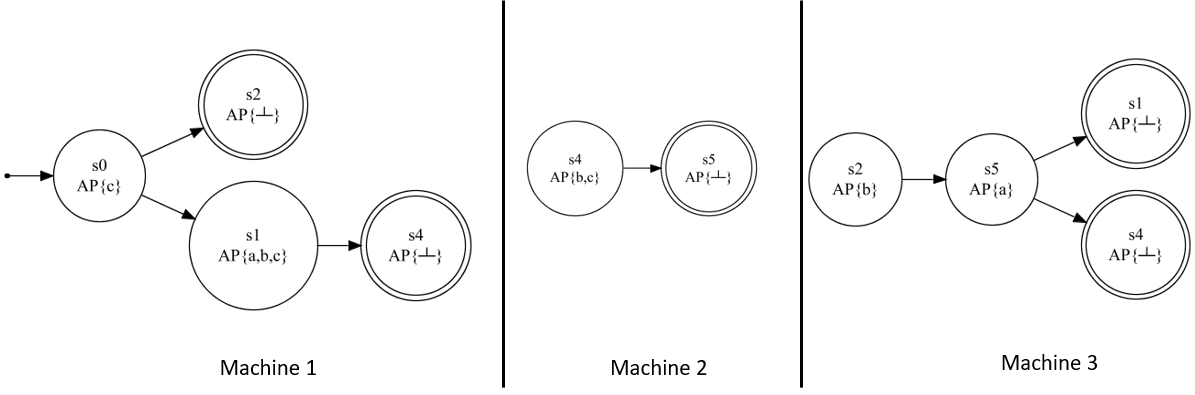
\includegraphics[scale=0.7]{img/stkd.png}
	\captionof{figure}{Structure de Kripke distribuée de cinq états, avec trois propositions} \label{stkrdpd}
 \end{center}
\section{Logique temporelle arborescente (CTL)}
Logique temporelle définie des opérateurs permettant de \s{lier} des variables propositionnelles \emph{p} aux instants \emph{t}. Par exemple, une assertion liée au comportement d'un programme telle que \s{après exécution d'une instruction i, le système se bloque}, les actions de cette assertion s'exécutent suivant un axe de temps : à l'instant \emph{t}, exécution de l'instruction \emph{i}, et à \emph{$t + 1$} blocage du système. La logique du temps arborescent permet de modéliser les expressions du passé et du futur \citep{Bakker1983}, \citep{Clarke1981}, \citep{Emerson1983}.\\

La logique du temps arborescent (CTL) « Computation Tree Logic (en aglais) » permet d'exprimer des propriétés portant sur les arbres d'exécution (issus de l'état initial) du programme. Elle modélise des expressions du passé et du futur à partir d'un état du système. Une expressions CTL exprime des propriétés relatives à l'arbre d'exécution grâce une syntaxe et une sémantique.

\subsection{Syntaxe de CTL}
Le langage des formules de CTL sont les formules d'état définies inductivement par:
\begin{itemize}
	\item  $ \forall p \in AP$, p est une formule d'état;
	\item  Si p, q sont des formules d'état, alors $p \vee q$ et $\neg p$ sont des formules d'état;
	\item Si p est une formule de chemin, alors \emph{$E_p$} et \emph{Ap} sont des formules de chemin;
	\item Si p et q sont des formules d'état, alors \emph{$X_p$} et \emph{pUq} sont des formules d'état.
\end{itemize}

\subsection{Sémantique de CTL}
La sémantique de CTL est interprétée dans une structure de Kripke. Les états sont décorés par les propositions atomiques ${\displaystyle p}$.\\
Soit $q_0$ un état de S. La sémantique de CTL est définie inductivement par:
\begin{itemize}
	\item  $p \in AP$, $q_0 \models p \Leftrightarrow p \in L(q_0 )$
	\item $q_0 \models p\vee q \Leftrightarrow q_0 \models p\; ou\; q_0 \models q$
	\item $q_0 \models \neg p \Leftrightarrow not(q_0 \models p)$
	\item  $q_0 \models Ep \Leftrightarrow  \exists \delta =q_0 …q_n$ telle que $\delta \models p$ (p formules de chemins)
	\item $q_0 \models Ap \Leftrightarrow \forall \delta =q_0 …q_n$ on a $\delta \models p$ (p formules de chemins)
	\item$ \delta \models Xp \Leftrightarrow \delta _1 \models p$ (p formules d'état)
	\item $ \delta \models pUq \Leftrightarrow \exists j \geq 0, \delta _j \models q\; et (\forall k <j, \delta _k \models p)$ (p et q formules d'état)
\end{itemize}
les opérateurs temporels sont définies par:
\begin{itemize}
	\item A (All), E (Exist): quantifications sur toutes les exécutions possibles à partir de l'état courant
	\item X (next), F (eventually), G (always),U précédent directement  A, E
	\item $\neg , \vee, \wedge$
\end{itemize}

Pour illustrer l'utilisation de la logique temporelle arborescence dans la formalisation des problèmes pratiques, nous donnons l'exemple du publiphone qui consiste à modéliser les actions qu'un utilisateur exécute pendant l'opération de tentative de téléphoner jusqu'à la fin de la communication. La procédure téléphonée est la suivante :
\begin{itemize}
	\item L'utilisateur doit décrocher le téléphone;
	\item Le système affiche insérer une carte;
	\item L'utilisateur insère une carte;
	\item Le système affiche le nombre d'unités restantes;
	\item L'utilisateur compose son numéro de téléphone avec la possibilité de le corriger pour obtenir le   bon numéro dans un délai de 2 secondes;
	\item L'utilisateur communique avec son correspondant, tant qu'il lui reste des unités. – Si la carte est épuisée, l'utilisateur a 10 secondes pour la changer;
	\item Lorsque la communication est terminée, l'utilisateur raccroche le téléphone;
	\item Le système affiche retirer la carte. – L'utilisateur retire sa carte;
\end{itemize}
Ensuite, formalisons les propositions atomiques :
\begin{itemize}
	\item u\_décrocher : l'utilisateur décroche le téléphone
	\item sys\_affiche(message) : le système affiche le message
	\item u\_insérer\_carte : l'utilisateur insère une carte
	\item u\_compser\_no : l'utilisateur compose le numéros
	\item u\_correction\_no : l'utilisateur corrige le numéros
	\item numéros\_correct : le numéros est correct
	\item u\_communiquer : l'utilisateur communique avec son correspondant
	\item u\_changer\_carte\_vide : l'utilisateur change sa carte qui est épuisée
	\item u\_raccrocher : l'utilisateur raccroche le téléphone
	\item u\_retirer\_carte : l'utilisateur retire sa carte
	\item ctl\_téléphoner : établit la clause de l'activité téléphoner
\end{itemize}

Enfin, on obtient la formalisation en CTL:\\

$u\_decrocher \; \wedge\; u\_inserer\_carte \wedge 	\\
AX [(u\_composer\_no\; \wedge\; EF (u\_reprise\_sur\_erreur)) \wedge \\
AX ((u\_communiquer \;\wedge\; EF (changer\_carte\_vide)) U \\
(u\_raccrocher \;\wedge \; u\_retirer\_carte))] \Rightarrow \; ctl\_telephoner$
\section{Model checking}
Le model checking peut-être ramené à la vérification d'une propriété \emph{P} sur un système $\phi : \phi \models P$. Plusieurs types de propriétés peuvent être vérifiés tels que les propriétés de sûreté ou de vivacité. Toutefois, vérifier des propriétés de sûreté est très souvent suffisant : On peut détecter des interblocages, vérifier des bornes ou encore qu'une section critique est bien respectée par les processus y accédant. 


Vérifier une propriété de sûreté revient à parcourir les états que peut atteindre un système, et pour chaque état rencontré, vérifier si la propriété est respectée. Il s'agit donc d'un parcours de graphe (en largeur ou en profondeur).

Ainsi, la génération distribuée de l'espace d'états permet de répartir l'ensemble des états entre les machines du réseaux, ce qui permet de pallier au problème de l'explosion combinatoire de l'espace d'états. Le but de cette génération distribuée est la vérification de systèmes de tailles importantes. De ce fait, les algorithmes de vérification feront aussi l'objet de distribution. 

L'algorithme de model checking distribué qui a été développé dans \citep{depriester2011bouneb}, elle représente un version simplifiée de l'algorithme de model checking distribué. Toutes les machines contribuent pour la vérification des propriétés exprimées en CTL. Chaque machine vérifiée la propriété sur la structure de Kripke partiale, la vérification au niveau des états à parties inconnues est traité indécidable. Ainsi, les machines coopèrent afin de vérifier la formule CTL. 

Dans cette section, nous présentons L'algorithme de model checking distribué qui a été proposer dans \citep{depriester2011bouneb}.

\subsection{Model checking CTL  sur les fargments}
Soit $M = (S, L, R, I)$ un fragment de structure de Kripke et une formule de CTL, l'algorithme récursif suivant calcule l'ensemble des états $H(f) \subseteq S$ qui satisfont f ou elle peut satisfaire f et qui exclut tous les états qui ne satisfont pas f. 
 \begin{flalign}
    \label{eqn1}
	&  T(p)= \left\{ x \in S\mid(x,p)=true\right\}&  \\
	\label{eqn2}
	&  U(p) = \left\{ x \in S\mid(x,p)=\bot\right\} \\
	&  F(p) = \left\{ x \in S\mid(x,p)=false\right\} \label{eqn3}
\\
	&  pour \; x \;\in T,inT(x) = (1,x) \label{eqn4}
\\
&	T^+(p)=\left\{ inT(x)\mid \forall x \in T\right\}\label{eqn5}
\\
&	pour \; x\; \in U,inU(x)=(-1,x) \label{eqn6}
\\
&	 U^+(p)=\left\{ inU(x)\mid \forall x \in U\right\}\label{eqn7}
\\
&	pour \;x \; \in F,inF(x)=(0,x) \label{eqn8}
\\
&	F^+(p)=\left\{ inF(x)\mid \forall x \in F\right\}\label{eqn9}
\\
&	S^+(p)=T^+(p)\cup U^+(p)\cup F^+(p)\label{eqn10}
\\
&	H(p)=T^+(p)\cup U^+(p); \;p\; une\; proposition\; atomique\label{eqn11}
\\
&	H(\ne f)=\left\{ inT(x)\mid x\in (S-map(snd,H(f)))\cup U^+(f)\right\}\label{eqn12}
\\
&	H(f\wedge g)=H(f)\sqcup H(g) \label{eqn13}
\\
&	H(f\vee g)=H(f)\sqcap H(g)\label{eqn14}
\\
&	H(AXf)=\left(\left\{inT(snd(e))\: \mid \forall\; e \; \in S^+(f).succ(e) \;\subseteq\; T^+(f)\; \subseteq\; H(f) \right\} \;\cup\atop \left\{inU(snd(e))\: \mid \forall \;e\; \in S^+(f).succ(e)\; \subseteq\; (T^+ (f)\;\cup\atop U^+(f))\; and\; \exists \;e' \;\in \;succ(e) \;telque\: e'^+(f)\right\}\right)\atop \sqcup\left\{inU(x) \mid x \in border(M) \right\}\label{eqn15}
\\
&	H(EXf)=\left(\left\{inT(snd(e))\: \mid \forall\; e' \; \in S^+(f).succ(e) \;\subseteq\; T^+(f) \right\} \;\cup\atop \left\{inU(snd(e))\: \mid \forall \;e'\; \in S^+(f).succ(e)\; \subseteq\; U^+(f)\subseteq\; H(f)\right\}\right) \sqcup\atop\left\{inU(x) \mid x \in border(M) \right\}\label{eqn16}
\\
&	H(AGf)=vZ.((H(f)\sqcap AXZ) \label{eqn17}
\\
&	H(AFf)=\mu Z.(H(f)\sqcup AXZ)\label{eqn18}
\\
&	H(A(f\cup g)=\mu Z.(H(g)\sqcup H(f))\label{eqn19}
\end{flalign}

Après l'application de l'algorithme récursif ci-dessus, nous avons $\forall s \notin H(f) \Rightarrow L(s, f) =false$. Les autres opérateurs, comme par exemple $EG$ peuvent être déduites de l'ensemble des opérateurs cités ci-dessus, par exemple $H(EGf) = H( \neg (AF \neg f))$.

\subsection{Model checking CTL  distribué}
l'algorithme model checking distribué considère l'ensemble de la formule \\$\phi \in \{ f EGf, AGf, AFf, EFf, A(fUg), E(fUg) \}$ peut-être vérifiée dans les états border et aussi la vérité sur les états border est le paramètre passé au transformateur de
prédicat  comme suit :

 \begin{flalign}
 & Y =  \{ s \in  border(M) \mid  L(s, \phi) = True ou L(s, \phi) = \bot \} \phi \; est \; une \; formule  &\\
 & AFp = \lambda Y. \mu Z.(p \vee Y \vee  AXZ)\\
 & AGp = \lambda Y.\mu Z.(p \vee Y \wedge  AXZ)  \\
 & EGp = \lambda Y.\mu Z.(p \vee Y \wedge EXZ) \\
 & A(p \cup q) = \lambda Y.\mu Z.(q \vee Y \vee(p \wedge AXZ)) \\
 & E(p \cup q) = \lambda Y.\mu Z.(q \vee Y \vee (p \wedge EXZ)) \\
\\
\end{flalign}

\emph{Y} représente l'absence d'information sur l'état border, grâce  à l'information obtenue au niveau des états border,  la validitée de la formule peut être conclus sur toute la structure de Kripke.
\section{Conclusion}{
Dans ce chapitre, nous avons présenté les réseaux de Petri ainsi que les systèmes de transitions étiquetées et aussi la structure de Kripke. Ensuite nous avons présenté  la logique temporelle arborescente et le model cheching distribué qui exploite l'information au niveau des états du graph ainsi qu'il permet la vérification malgré l'insuffisance d'information résultante de la distribution de l'espace d'états sur plusieurs nœuds.		
 	\part{Contributions}
	\clearpage
		%%%%%%%%%%%%%%%%%%%%%%%%%%%%%%%%%%%%%%%%%%%%%%%%%%%%%%%%%%%%%%%%%%%%%%%%%%%%%%%%%%%%%%%%%%%%%
%%									Chapitre Contribution											%
%%%%%%%%%%%%%%%%%%%%%%%%%%%%%%%%%%%%%%%%%%%%%%%%%%%%%%%%%%%%%%%%%%%%%%%%%%%%%%%%%%%%%%%%%%%%%
\chapter{Algorithme de distribution d’espace d’états basée sur le comportement des systèmes}
%	\citationChap{
%	...
%	}{...}

%%%%%%%%%%%%%%%%%%%%%%%%%%%%%%%%%%%%%%%%%%%%%%%%%%%%%%%%%%%%%%%%%%%%%%%%%%%%%%%%%%%%%%%%%%%%%
 \section{Introduction}
Dans \citep{Saidouni2012}, \citep{TabibSaidouni2016}, \citep{BENSETIRA2017}, nous avons constaté que les méthodes de génération des espaces d’états pour le model checking consiste  qu’un grand espace d'états non structuré soit divisé en parties de tailles équilibrées, de telle sorte que peu de transitions lient les différentes  parties, car chaque transition externe peut entraîner une surcharge de communication.

Après une étude des espaces d'états générés, nous avons constaté que la diminution de transitions liant les différentes parties peut entraîner un mauvais équilibrage de charge entre les machines du réseau. Outre l’équilibrage de charge, il peut entraîner une mauvaise qualité de distribution de l'espace d'états car lorsqu'une formule du model checking n'est pas vérifiée sur un état la diminution de transitions externes n'empêche pas une surcharge de communication. La qualité de distribution est estimée en fonction de la quantité de communication requise pour l’exécution des tâches distribuées \citep{EzekielLuttgen2008}. Ainsi la réalisation de ces objectifs nécessiterait des informations supplémentaires sur l’espace d’états considéré et les communications engendrées. 

Ces raisons nous ont amené à proposer une nouvelle approche de distribution qui vise à analyser le comportement d’un système donné en générant son espaces d’états et en extrayant les informations pertinentes sur les états et leurs connexions (transitions internes et externes). Ensuite, redistribuer les états pertinents selon une stratégie comportementale de la théorie de jeux afin d’optimiser les performances du système. Les machines sont considérées comme des joueurs, chaque machine cherche à optimiser ces performances en définissant une bonne localité pour un état pertinent tout en optimisant l’équilibre de charge et la quantité de communications entre les machines.
 
Dans ce qui suit nous présentons la nouvelle politique de redistribution de l’espace d’états basée sur le comportement du système ainsi que les résultats obtenus. 
 

\section{Politique de distribution de l’espace d’états basée sur le	comportement du système}
 
La politique proposée \emph{\BbSSD{}}, vise à optimiser la distribution de l’espace d’états ainsi le temps de vérification du model checking. Pour un système donné spécifier a partir d'un réseau de Petri, nous utilisons un algorithme de génération parallèle pour construire la structure de Kripke distribuée, en utilisant la fonction \emph{MD5} pour le partitionnement de l’espace d’états entre les machines du réseau. Après cela, lors de l'exécution du model checking, chaque machine analyse son fragment (structure de Kripke partiale) et élabore certaines statistiques sur les états par rapport a la vérification. Les statistiques  générer sur chaque état mesure la dépendance de l'état par rapport aux états de la machine local ou aux états des machines distantes. Une fois le processus de vérification du model checking est terminé, Le protocole de redistribution peut être lancer afin de calculer pour chaque état \emph{Externe} et \emph{soliciter} sur lesquels la formule n'est pas vérifiée l'ensembles des états à déplacer et à dupliquer. Après le calcul des ensembles on décide, sur la base de l'écart minimum et maximum des états a stocké sur la machine, si l'ensemble peut être déplacer ou rester dans une machine afin de minimiser la quantité de communication entre les machines avec une bonne distribution, ainsi les transitions externes peut être réduit.
L’algorithme général est l'Algorithme \ref{bbssd} :\\
\begin{algorithm}[H]\label{bbssd}
	\SetAlgoLined
	\SetKwIF{If}{ElseIf}{Else}{if}{then}{else if}{else}{endif}
	 Générer la structure de Kripke distribuée à partir de la spécification d'un réseau de Petri\;
	 Exécution du model checking et élaboration des statistiques sur chaque état\;
	 Redistribuer des états, en optimisant les performances du système\;	  
	\caption{\BbSSD{}}
\end{algorithm}

Dans les sections suivantes, nous détaillons les phases de cet algorithme.

\subsection{Génération de l’espace d’états distribuée à partir de la spécification d'un réseau de Petri}{
La spécification du réseau de Petri est faite à partir d'une machine choisie aléatoirement. Le processus de génération de l'espace d'états distribuée est fait par l’exploration de l’état initial en générant tous ses états successeurs. Par la suite, toutes les machines disponibles sur le réseau contribuent à la construction des fragments de l’espace d’états distribué. Pour chaque nouvel état généré appartenant à une machine $M_i$, tous ses états successeurs sont générés. Un état successeur peut être dans la même machine ou dans une machine distante. Chaque machine $M_i$ envoie tous ses états externes aux machines déterminées par la fonction de partition. La fonction de partition est basée sur la fonction de hachage cryptographique \emph{MD5} qui renvoie un index $j\;(j \in 0, N-1)$. La fonction de hachage adoptée réalise un bon équilibrage de charge entre les $N$ machines du réseau.  La génération distribuée se termine lorsqu'il n'y a aucun états en attente d'être exploré.\\
L’algorithme de génération de l’espace d’états distribuée est l'Algorithme \ref{gendistribuer} :\\
\SetKwFunction{printlcs}{}
\begin{algorithm}
	\SetAlgoLined
	\SetKwIF{If}{ElseIf}{Else}{if}{then}{else if}{else}{endif}
	\SetAlgoLined	
	\SetKwInOut{Mi}{$M_i$}
	\SetKwInOut{Mj}{$M_j$}
	\SetKwInOut{etati}{$Etat_i$}
	\SetKwInOut{ei}{$E_i$}
	\SetKwInOut{si}{$S_i$}
	\SetKwInOut{t}{$t$}
	\SetKwInOut{T}{$T$}
	\SetKwInOut{smm}{$s,m,m'$}
	\SetKwInOut{tb}{$t_b$}
	\SetKwInOut{sm}{$s.m$}
	\SetKwInOut{sprp}{$s.L$}
	\SetKwInOut{te}{$TExplore$}
	\SetKwInOut{tr}{$TR_i$}
	\SetKwInOut{Pres}{$Pres$} 
	\SetKwInOut{Post}{$Post$}
	\SetKwInOut{pps}{$Prop\_Pres$}
	\SetKwInOut{ppt}{$Prop\_Post$}
	\AlgoDontDisplayBlockMarkers\SetAlgoNoEnd\SetAlgoNoLine%
	\Mi{machine i}
	\Mj{machine j}
	\etati{\{dehors,dedans\}}
	\ei{init à $\emptyset$, pile des états non encore explorés appartenant à la machine i}
	\si{init à $\emptyset$, la liste des états déjà explorés appartenant à la machine i }
	\smm{un état}
	\sm{marquage d'un états}
	\sprp{liste des propriétés d'un états}
	\tr{la liste des relations de transitions de la machine i}
	\T{a liste de transitions}
	\tb{transition bloquant}
	\te{liste transition admissible}
	\t{une transition}
	\Pres{matrice pres du réseau de Petri}
	\Post{matrice post du réseau de Petri}
	\pps{matrice pres des propriétés}
	\ppt{matrice post des propriétés}

	 \caption{Génération Initiale Distribuée}\label{gendistribuer}
\end{algorithm}

\begin{algorithm}
	\LinesNumbered
	% This is to restore vline mode if you did not take the package as \usepackage[linesnumbered,ruled,vlined]{algorithm2e}
	\SetAlgoVlined 
	\SetKwFunction{algo}{}\SetKwFunction{proc}{proc}
	\Begin{	 
	 \SetKwProg{myalg}{Reception Etat}{}{}
	 
	 \myalg{\algo{m:etat}envoyé par $M_j$}{  
	 	$s\leftarrow findByMarquage(m,S_i)$\;	
	 	\uIf{($ s ==null$)}{
	 		$m.sub\leftarrow\{ M_j \}$\;
	 		Empiler(m,$E_i$)\;	 		
	 		\If{($Etat_i$!= dedans)}{
	 			GenerationDistribue$_i$()\;
 			}
	 	}
 		\Else{
 		   ajouter $M_i$ à la liste des machines de l'etat portant identifiant \emph{m} \;			
 		}	 		  		
	 }{} 	  	
   	\SetKwProg{myalgone}{GenerationDistribue$_i$}{}{}   
  	 \myalgone{\algo{}}{  
	  	$Etat_i\leftarrow dedans$\;	
	  	\While{($ E_i !=\emptyset$)}{
	  		$m\leftarrow depiler(E_i)$\;
	  		$TExplore \leftarrow \{t\in T\mid m.m[t>\}$\;
	  		$S_i\leftarrow S_i \cup \{m\}$\;
	  		\ForEach{($t \in TExplore$)}{
	  			$m'.m\leftarrow m.m + Post(t)-Pres(t)$\; 
	  			$m'.L\leftarrow m.L + Prop\_Post(t)-Prop\_Pres(t)$\; 
	  			$M_j \leftarrow MD5(m'.m)$\;
	  			\uIf{$M_j = =M_i$}{
	  				$s\leftarrow findByMarquage(m,S_i)$\;
	  				\If{(findByMarquage(m'.m,$S_i$)==null and findByMarquage(m'.m,$E_i$)==null)}{
	  					Empiler(m',$E_i$)\;
	  				}
  				}\Else{  				
  					Envoyer (m') à $M_j$\;
  				}
  				$TR_i\leftarrow TR_i\cup \{(m,t,m')\}$	\;
  			}	
	  			
	  		\If{(TExplore== $\emptyset$)  }{
	  		 	$TR_i\leftarrow TR_i\cup \{(m,t_b,m)\}$\;
	  		}
  		}
	  	$Etat_i\leftarrow dehors$\;
	  }{}
  }
 	 \SetKwProg{myalgone}{Initialisation}{}{ }
  	 \myalgone{\algo{}}{  
  	 $T\leftarrow init$\;
  	 $Pres\leftarrow init$\;
  	 $Post\leftarrow init$\;
  	 $Prop\_Pres\leftarrow init$\;
  	 $Prop\_Post\leftarrow init$\;
  	 $m.m\leftarrow init$\;
  	 $m.prop\leftarrow init$\;
  	 $M_i \leftarrow MD5(m.m)$\;
  	 Envoyer (m) à $M_j$\;
  
  }
	
\end{algorithm} 
}
\pagebreak
\input{contribution/Section1}
\input{contribution/Section2}
\input{contribution/Section3}
\input{contribution/Section4} 
%%%%%%%%%%%%%%%%%%%%%%%%%%%%%%%%%%%%%%%%%%%%%%%%%%%%%%%%%%%%%%%%%%%%%%%%%%%%%%%%%%%%%%%%%%%%%
%%									section Algorithmes	de Redistribution						%
%%%%%%%%%%%%%%%%%%%%%%%%%%%%%%%%%%%%%%%%%%%%%%%%%%%%%%%%%%%%%%%%%%%%%%%%%%%%%%%%%%%%%%%%%%%%%
\makeatother

%L'algorithme de \mcd{} est formalisé comme suit:

	%\begin{fleqn}

%\end{fleqn}

%%%%%%%%%%%%%%%%%%%%%%%%%%%%%%%%%%%%%%%%%%%%%%%%%%%%%%%%%%%%%%%%%%%%%%%%%%%%%%%%%%%%%%%%%%%%%
%%									sub section Initialisation de $\beta ,\gamma $				%
%%%%%%%%%%%%%%%%%%%%%%%%%%%%%%%%%%%%%%%%%%%%%%%%%%%%%%%%%%%%%%%%%%%%%%%%%%%%%%%%%%%%%%%%%%%%%

\subsection{Calcul des valeurs des parametres $\parametretwo{} \; et\;\parametretree{} $ }
 
{L'initialisation des paramètres s'effectue lors de l'exécution du \mc{}. Tel que nous l'avons souligné, ces paramètres  sont initialisés à partir des états sur lesquels la formule n'est pas vérifiée. Par la suite, les états liés sont marqués par chaque état dont ils dépendent (dans l'algorithme c'est la variable \textbf{f} qui stocke cet ensemble d'états). Enfin, les états liés sont énumérés. Un état est dit lié, lorsque la formule n'est pas vérifiée sur ses successeurs directs ou indirects. Certains prédécesseurs directs ou indirects ne sont pas liés aux successeurs directs ou indirects sur lesquels la formule n'est pas vérifiée car celle-ci n'est pas vérifiée sur ces prédécesseurs. Cela motive la duplication de ces états prédécesseurs. A titre d'exemple, l'exécution de la formule  \textit{$AG(a)$} sur la structure de Kripke de la Figure(\ref{skd2}), l'état \sneuf{} est un prédécesseur indirect de l'état \s{S14}, celui-ci peut être dupliqué sur une autre machine car la vérification de la formule sur cet état est indépendante des autres états. 

Dans ce qui suit nous proposons la démarche d'initialisation des paramètres, le marquage des états liés, l'énumération des états liés et des états à dupliquer. Cette démarche est ajoutée à l'algorithme de model checking définit ci-dessus.
}
	\mysubsection{Initialisation des paramètres $\parametretwo{}$  et $\parametretree{} $ }{
Les paramètres $\parametretwo{}$ et $\parametretree{}$ sont initialisés à zéro au niveau des états qui ne comportent pas la formule à vérifier. Lorsque l'état appartient à la machine, le paramètre $\parametretree{}$ sera initialisé à $1$, cela signifie que cet état peut être dupliqué dans les machines qui le référencent. Par exemple, l'exécution de la formule  \textit{$AG(a)$} sur la structure de Kripke distribuée de la Figure(\ref{skd2}) fait qu'à l'état \sneuf{}, le paramètre $\parametretree{}$ est initialisé à 1 pour marquer la duplication de cet état. On remarque que la duplication de l'état \sneuf{}  sur la \mone{}, permet de réduire le temps de vérification de la formule, car la valeur logique de la formule sur à l'état \sneuf{} est connue, la \mtwo{} n'envoie pas alors de message concernant la valeur logique de la formule sur cet état. Le principe d'initialisation est formalisé sur l'équation (\ref{eqn3}). On obtient alors:

\input{contribution/Algorithm1}
}
\mysubsection{Marquage des états liés}{
Pendant l'exécution de l'algorithme de vérification, la valeur logique de la formule sur certains états peut dépendre des successeurs directs ou indirects, ces états sont alors liés. La formule peut être vérifiée sur les successeurs, ils peuvent appartenir à d'autres machines. Lorsque la formule n'est pas vérifiée sur un état successeur, les états liés sont alors marqués par cet état. Le principe de marquage est implémenté sur les deux algorithmes de base du model checker. Ils sont définis comme suit : 
\begin{description}
\item[Premier algorithme :] Il est défini par l'équation (\ref{eqn15}), il est utilisé lorsque la vérification concerne tous les successeurs. Ainsi Lorsque la formule n'est pas vérifiée au niveau d'un successeur, deux cas se présentent : 
	\begin{itemize}
		\item La propriété est vérifiée sur l'état, l'état est alors lié à un successeur. Les successeurs sur lesquels la formule n'est pas vérifiée sont marqués sur l'état.
		\item Lorsque la propriété n'est pas vérifiée sur un état, celui-ci peut être dupliqué soit sur la machine réalisant le traitement soit sur des machines distantes. Les états successeurs sur lesquels la formule n'est pas vérifiée sont enregistrés dans l'ensemble \s{limit}, cela signifie que cet état est indépendant de ses successeurs et peut donc être dupliqué sur des machines distantes. Sur l'exemple (\ref{ea1}) de l'Algorithme(\ref{alg1}), la valeur logique de la formule à l'état \s{S9} est indépendante des états \s{S14} et \s{S7}. L'état \s{S9} peut alors être dupliqué sur les machines qui possèdent ses prédécesseurs.
	\end{itemize}  
   
\item[Deuxième algorithme :] Il est défini par l'équation(\ref{eqn16}). Il se différencie du premier algorithme par la vérification de la formule sur les successeurs. Il vérifie l'existence de la propriété sur un successeur. 
\end{description}
En plus des conditions des algorithmes, l'existence de l'itération courante est vérifiée. Cette condition permet de marquer les états de cette itération. Ce principe est formalisé comme suit:\\
\input{contribution/Algorithm2}\break
} 
\mysubsection{Énumération des états liés}{
Après le marquage des états, on obtient sur les états liés les états dont ils dépendent. Ainsi pour chaque état dépendant, les états qui lui sont liés sont énumérés, cela permet d'attribuer des valeurs aux paramètres $(\parametretwo{}$ et $\parametretree{})$. L'attribution des valeurs peut concerner les états appartenant à la machine locale ou appartenant aux machines distantes. Ces valeurs permettent d'effectuer un redéploiement des états sur la bonne machine. Selon le type de chaque état la technique d'énumération est la suivante:
\begin{description}
\item[\ee{} :] Les états externes(\s{border}) sont des états appartenant aux machines distantes. Lorsque la formule n'est pas vérifiée sur ces états, le nombre d'états liés sont recensés. La valeur calculée est attribuée au paramètre $\parametretwo{}$ de l'état \s{border}. 
Dans l'exemple(\ref{ea2}), la valeur du paramètre $\parametretwo{}$ est égale à $2$ à l'état \s{S22} de la \mtwo{}.
 Ainsi la valeur du paramètre $\parametretree{}$ correspond au nombre d'états pour lesquels l'état \s{border} a été inséré dans leurs ensembles respectifs \s{limit}. Dans le cas des états externes, la duplication de ces états sur une machine donne une structure de Kripke incohérente (la structure obtenue présente des états dupliqués sans aucuns prédécesseurs sur la machine elle même, ce modèle est alors incohérent vis à vis d'une structure de Kripke). Pour obtenir une structure cohérente il est envisageable de déplacer ces états sur d'autres machines tout en laissant les duplicatas sur la machine local. Pour ce faire le paramètre$\parametrefour{}$ est utilisé pour stocker le nombres de ces états à la place du paramètre $\parametretree{}$. La valeur de ce paramètre est calculée similairement  à celle du paramètre $\parametretree{}$.
 L'application de ce principe sur l'exemple(\ref{ea2}) permet d'attribuer la valeur $1$ au paramètre $\parametrefour{}$ à l'état \s{S22} de la \mtwo{}, car cet état est stocké dans l'ensemble \s{limit} de l'état \s{S14}.  
 
\item[\ei{} :]  Les états internes sont des états appartenant à la machine locale. Lorsque ces états disposent des prédécesseurs directs sur d'autres machines distantes, les valeurs des paramètres sont alors calculés. La valeur du paramètre $\parametretwo{}$ correspond aux nombres des successeurs directs et indirects présents entre les état marqués sur l'ensemble de dépendance (la variable \s{\textbf{f}}) de l'état, ce nombre est incrémenté de $1$ car l'état dépend de ces états l'à. Par contre la valeur du paramètre $\parametretree{}$  correspond aux nombre des états internes présents sur l'ensemble de dépendance.
  L'application de ce principe sur l'exemple(\ref{ea2}) permet d'obtenir la valeur $2$ pour le paramètre $\parametretwo{}$ et $0$ pour le paramètre $\parametretwo{}$ à l'état \s{S7} de la \mtwo{}.  
\end{description}

Ces principes sont formalisés comme suit:
\input{contribution/Algorithm3}
}

\mysubsection{Échange des valeurs des paramètres}{
Après le calcul des valeurs des paramètres, ces valeurs sont envoyées aux machines concernées par l'état. A la réception des valeurs, ces dernières sont stockées sur l'état concerné. Ce prince est formalisé comme suit:
\input{contribution/Algorithm4}
}
%%%%%%%%%%%%%%%%%%%%%%%%%%%%%%%%%%%%%%%%%%%%%%%%%%%%%%%%%%%%%%%%%%%%%%%%%%%%%%%%%%%%%%%%%%%%%
%%									subsection Algorithmes	de Redistribution						%
%%%%%%%%%%%%%%%%%%%%%%%%%%%%%%%%%%%%%%%%%%%%%%%%%%%%%%%%%%%%%%%%%%%%%%%%%%%%%%%%%%%%%%%%%%%%%
\subsection{Algorithme de Redistribution }
 
Après l'envoi des valeurs calculées, les états \emph{Border et Notifier} présentent les valeurs calculées aux paramètres $\parametretwo{}$ et $\parametretree{}$ par la machine locale et les machines distantes. Ces valeurs permettent d'appliquer une stratégie de redistribution des états. La stratégie adoptée est celle d'un jeux non coopératif. Chaque machines cherche a optimisée le temps de calcul de la vérification d'une formule en se focalisant sur l'information que pressente les valeurs calculées par chaque machine. Ainsi, grâce à ces valeurs, sur une machine est calculé calcule l'ensemble minimal des états à envoyer sur une machine distante ainsi que l'ensemble minimal des états à recevoir par cette machine locale. L'envoi des états nécessite la prise en compte de l'équilibrage de charge.  
Dans ce qui suit nous proposons une stratégie de recherche de ces ensembles minimaux d'états à déplacer, dans un sens ou dans l'autre, suivi d'une technique d'envoi de ces ensembles d'états.

\mysubsection{Recherche de l'ensemble minimal des états à importer}{
Dans cette partie l'algorithme permet de chercher sur les valeurs des paramètres $\parametretwo{}$ et $\parametretree{}$  calculées par les machines distantes le couple minimal. Le nombres des états associés à ce couple doit être inférieur au nombre des états associés au couple calculé par la machine locale. Le déplacement de ces états sur une machine distante permet de diminuer le temps de la vérification car l'algorithme détecte la valeur logique de ces états sans qu'une notification ne soit envoyée. Ainsi, le couple minimal est recherché sur les valeurs envoyées par les machines distantes au niveau des états \bn{}, comparées aux valeurs  calculées par la machine sur cet état.  Le couple minimal est celui qui dispose des plus petites valeurs des paramètres calculées  par la machine local sur ces états. Cette recherche est faite en premier temps sur les états ayant une dépendance mutuelle (c'est-à-dire les états distants dépendant l'un de l'autre) car le regroupement de ces états sur une machine diminue le nombre d'itérations de deux. Ainsi, lorsqu'il n'existe pas une dépendance mutuelle entre les états le couple minimum est recherché sur les valeurs envoyées par les machines distantes au niveau des états \bn{}. La formalisation de ce principe est la suivante: 
\input{contribution/Algorithm_Search_StatesToImport}
\nopagebreak
}

\mysubsection{Recherche de l'ensemble minimal des états à déplacer}{
L'ensemble minimal des états à déplacer d'une machine distante correspond au couple minimum des couples($\parametretwo{}$ et $\parametretree{}$) calculés par la machine locale sur les états(\bn{}). Le couple minimum représente la plus petite valeur obtenue au paramètre $\parametretwo{}$ avec une valeur minimale au paramètre $\parametretree{}$. Les états associés à ce couple entrainent un léger déséquilibre qui pourrait être accepté avec l'écart calculé. La recherche de ce couple ($\parametretwo{}$ et $\parametretree{}$) est formalisée comme suit:

\input{contribution/Algorithm_Search_StatesToMove}
\nopagebreak
}

\mysubsection{Envoi d'une requête}{
Après la recherche de l'ensemble minimal des états à déplacer, ces états sont ensuite envoyés à la machine concernée sous forme de requête. La requête peut contenir des états à insérer sur la machine distante ou une demande de l'ensemble des états à déplacer sur la machine distante. Ainsi, l’envoi de la requête est fonction de l'équilibrage de charge.

\begin{itemize}
 \item  Lorsque le résultat de la différence entre le nombre des états à déplacer et le nombre des états à importer  est inférieur ou égale à l'écart calculé la requête envoyée comporte alors les états migrants de la machine locale et une demande des états de la machine distante.
 \item Sinon, si le nombre des états à déplacer est inférieur ou égale à l'écart calculé la requête comporte les états à insérer sur la machine distante.
 \item Sinon, s'il s'agit des états de la machine distante, la requête concerne ces états afin que la machine distante puisse les envoyer à la machine.
 \end{itemize}  
Ce principe est formalisé comme suit:
\include{contribution/Algorithm_SendResquest}
\nopagebreak\nopagebreak\nopagebreak
}
\mysubsection{Réception d'une requête}{
A la réception d'une requête les états à insérer sont insérés et les ensemble des états demandés sont envoyés. Lorsque des états sont insérés à la structure de Kripke d'une machine, les valeurs calculées par la machine distante sont alors mises à jour par celles correspondantes à la machine locale pour le bon fonctionnement du protocole. Après ce processus  l'Algorithme \ref{alg6} est relancé. 
Ce principe est formalisé comme suit:
\input{contribution/Algorithm_ReceveResquest}
\nopagebreak
}
\begin{Exemple}\label{ea5}
L'exécution du protocole de redistribution sur les résultats générés dans les exemples précédents permet d'obtenir  les résultats suivants:

\begin{description}
\item[Itération 1 :] Pendant la première itération du protocole sur la \mone{}, l'algorithme détecte que les état \s{S7} et \s{S9} sont mutuellement dépendants. Ainsi, les valeurs envoyées par la \mtwo{} sur l'état \s{S7} sont minimales, les états concernant ces valeurs sont à déplacer de la \mtwo{}. Ainsi les états à déplacer de la \mone{} vers la \mtwo{} sont recherchés, l'algorithme détecte que les états liés à l'état \s{S11} sont minimaux. Les états de cet ensemble sont à envoyer sur la \mtwo{}. Après ces deux processus de recherche, les valeurs sont évaluées afin de ressortir la requête à envoyer. L'évaluation montre qu'il est possible d'importer les prédécesseurs de l'état \s{S7} et les prédécesseurs de  l'état \s{S11}.
L'état \s{s2} ne sera pas envoyé parmi les états à déplacer car la \mtree{} possède des prédécesseurs directs de cet état. Après l'envoi des états à déplacer, la \mone{} possède l'état \s{S9}, quant à l'état \s{S1} il est possédé par la \mtwo{}.


Sur la \mtree{} l'algorithme détecte qu'il est possible de déplacer l'état \s{S22} sur la \mtwo{}.


   Après ces redistributions d'états, le protocole détecte qu'il est impossible de redistribuer les états car il risque d'avoir un déséquilibre de charge sur les machines.
   
\end{description}
\centering
	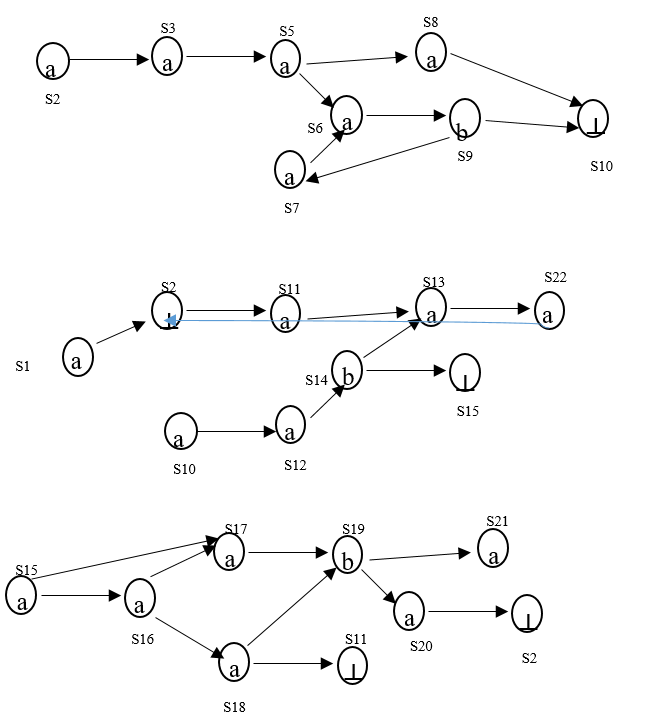
\includegraphics[height=5in]{img/Rskd.png}
	
	\captionof{figure}{Structure de kripke Redistribu\'{e}} 
\end{Exemple}
\section{Étude expérimentale}
Cette section présente les résultats expérimentaux obtenus en appliquant la méthode de redistribution proposée dans ce chapitre.

\subsection{Configuration de la mise en œuvre}
Nous avons développé l’outil qui génère une structure de Kripke distribuée. L’outil dispose d’un éditeur de graphique pour dessiner et modifier les systèmes analysés à partir d'un réseau de Petri (Figure \ref{apppetrinet}).

L’approche proposée a été implémenter avec le langage de programmation JAVA sur IDE IntelliJ, en utilisant le base de donnée orienté graphe Neo4J pour le stockage de l'espace d'états, le Docker pour l'hébergement de ces bases de données. le framework Java Agent Development est aussi utiliser pour faciliter la communication entre les machines.

\section{Conclusion}
Dans ce chapitre, nous avons présenté une nouvelle approche pour la distribution de l’espace d'états basée sur le comportement du système analysé. L’approche proposée vise à améliorer la distribution de l'espace d'états qui sera bénéfique pour le model checking car elle entraine moins de communications entre les machines. L’approche proposée analyse le comportement d’un système donné, et extrait les informations pertinentes sur ses états. Ensuite, les états sont redistribués suite à leurs pertinences soit migrés définitivement soit dupliqués sur d’autres machines, afin de minimiser le nombre de communications entre les machines. La machine réceptrice de ces états est choisie suite à une stratégie comportementale de la théorie jeux où chaque machine cherche à minimiser le taux de ses communications tout en maintenant un bon équilibrage des états entre les machines à l’aide des seuils prédéfinis pour chaque machine.

L’approche proposée peut être adoptée à tout autre spécification formelle ou modèles d'analyse de données car il est pratiquement possible de la formalisée comme un graphe. 		
	%%%%%%%%%%%%%%%%%%%%%%%%%%%%%%%%%%%%%%%%%%%%%%%%%%%%%%%%%%%%%%%%%%%%%%%%%%%%%%%%%%%%%%%%%%%%%
%%									Chapitre Conclusion
%%%%%%%%%%%%%%%%%%%%%%%%%%%%%%%%%%%%%%%%%%%%%%%%%%%%%%%%%%%%%%%%%%%%%%%%%%%%%%%%%%%%%%%%%%%%%
\chapter{Conclusion et Perspectives}
\section{Conclusion}

\section{Perspectives}
	
				
	\begin{appendix}
		\addcontentsline{toc}{part}{Bibliographie}
		\markboth{Bibliographie}{}
		\pagenumbering{Roman}	
		%\bibliographystyle{francaissc}
		%\bibliographystyle{dinat} 
		%\bibliographystyle{plainnm}
		\bibliographystyle{dinat}
		 \bibliography{Biblio}	
	
		
		%Imports the bibliography file "sample.bib"
	%\bibliography{sample}	
	\end{appendix}	
\end{document}
